\chapter{Sparse Component Analysis, data restoration and inpainting on the sphere}
\label{ch_sca_datarest}

\section{Morphological Component Analysis on the sphere}

A usual task  in processing signals, images as well as spherical data maps, is to decompose the data 
into its elementary building blocks. This can be formulated as an inverse problem where the data is 
assumed to have been generated according to the following model : 
\begin{equation}
 y = \sum_{i} \alpha_i \phi_i + \eta
\end{equation}
that is a linear combination of relevant waveforms $\phi_i \in \mathbb{R}^n$ with weights $\alpha_i$. 
Here $\eta$ represents possible contamination by additive, typically Gaussian white noise. Given data 
$y\in \mathbb{R}^n$, one then wants to recover the underlying structures that is to say estimate a set 
of waveforms $\phi_i$ that build the data and their corresponding weights $\tilde{\alpha}_i$. The solution 
to this estimation problem will depend heavily on the available prior information. Of interest here is 
the case where one is given a priori a set a waveforms from which to select a good subset. This set 
may be a basis, a frame or several bases or frames grouped into a large redundant dictionary.

Possible dictionaries in 1D and 2D include Fourier and related bases, wavelet bases, as well as 
other more recent multiscale systems such as the ridgelet~\citep{cur:candes99_1} and curvelet 
frames~\citep{cur:donoho99,starck:sta01_3}, etc. Depending on the morphology of the data, each of 
these dictionaries will have different performance characteristics 
%perform more or less efficiently 
in a non-linear approximation scheme. For instance, sparse approximations of piecewise smooth 
signals or images with point singularities are easily obtained using wavelets. However these 
are no longer optimal in the case of piecewise smooth images with singularities along smooth 
curves or edges. Such images are more efficiently approximated using curvelets which are highly 
anisotropic and thus exhibit high directional selectivity. Digital implementations of both ridgelet 
and curvelet transforms and their application to image denoising are described in~\citep{starck:sta01_3}.

\newpage
Available transforms in the spherical topology include the spherical harmonics and several 
wavelet transforms. Software packages such as Healpix\footnote {http://www.eso.org/science/healpix}~\citep{pixel:healpix} 
or Glesp~\citep{pixel:glesp} provide approximate digital spherical harmonic transform routines 
based on their specific pixelization schemes. Schr{\"o}der and Sweldens~\citep{wave:sweldens95a} 
have developed an orthogonal wavelet transform on the sphere based on the Haar wavelet function 
which then suffers from the poor frequency domain localization properties of the primitive Haar function 
%properties of the Haar function 
and from the problems inherent in orthogonal decomposition (e.g. lack of translation invariance). 
A few papers describe continuous wavelet transforms on the sphere~\citep{wave:antoine99bis,wave:cayon01,wave:holschneider96,wave:wiaux,bogdanova} 
which have been extended to directional wavelet transforms~\citep{wiaux06,wave:hobson04}. 
Although useful for data analysis, these continuous transforms lack an inverse transform and hence 
are clearly not suitable for restoration or synthesis purposes.

In their pioneering  work, Freeden and Maier~\citep{freeden02,freeden03} gave a wavelet transform 
and reconstruction scheme on the sphere which is based on the spherical harmonic transform. 
Following this idea, Starck et al.~\citep{starck:sta05_2} have proposed a new invertible 
isotropic undecimated wavelet transform (UWT) on the sphere which preserves the same desirable 
properties as the standard isotropic UWT for flat 2D maps~\citep{starck:book98}: the reconstruction 
is simple and immediate since it is just the addition of all the wavelet bands with the coarsest scale. 
Based on this new decomposition, other multiscale transforms such as the pyramidal wavelet transform, 
the ridgelet transform and the curvelet transform have been successfully constructed on the sphere \citep{starck:sta05_2}. 
%
Each of these decompositions on the sphere will sparsely represent parts of the image based 
on their morphological properties. Wavelets will easily detect more or less isotropic localized 
structures, while curvelets are better suited for efficiently detecting highly anisotropic objects.
%
% ,  based on the spherical harmonics decomposition, is to our knowledge the only one to have an inverse transform. This set of spherical transforms has recently been enriched with a new invertible  isotropic undecimated wavelet transform~\citep{starck:sta05_2} the properties of which are similar to those of the \emph{\`a trous} algorithm and with digital ridgelet and curvelet transforms on the sphere. These tools make it possible to detect both point singularities and  edges in spherical maps. 
%
%

A data set $y$ has an exact representation over any complete basis of the data space, or several 
such exact representations in the case of redundant overcomplete dictionaries. However, these 
representations are not equally interesting in terms of data modeling or feature detection. In fact, 
a strong a priori is to favor representations of $y$ that use only a small number of waveforms 
leading to a more concise and possibly more interpretable representation of the data. In fact, 
building sparse representations or approximations is the (he)art of structured data processing: 
the design of good detection, denoising, restoration and compression algorithms relies on the 
availability of good dictionaries and good selection algorithms. Indeed, selecting the smallest 
subset of waveforms from a large dictionary, that will linearly combine to reproduce the salient 
features of a given signal or image, is a hard combinatorial problem. Several pursuit algorithms 
have been proposed that can help build very sparse decompositions such as the greedy Matching Pursuit (MP)~\citep{wave:mallat93} 
algorithm which refines the signal approximation by picking at each iteration the one waveform 
which best correlates with the current approximation error. Basis Pursuit (BP) ~\citep{wave:donoho98} 
is a global procedure which seeks an approximation $\tilde{y}$ to $y$ by solving the linear programming problem:
\begin{equation}
\min_{ \alpha } ~ \|\alpha\|_{{ \ell_1}} \mbox{ subject to } y = \Phi \alpha.
\label{eqn_bp}
\end{equation}
where the ${\ell_1}$ norm measures sparsity in place of the ${\ell_0}$ counting norm. 

In the presence of noise, a noise-aware variant of BP, known as BPDN (for BP denoising), can be 
stated as a convex quadratic programming problem and solved using the Interior Point method 
\citep{wave:donoho98}. The BPDN problem can also be written in the augmented Lagrangian form:
\begin{equation}
\min_{ \alpha } ~  \|y - \Phi\alpha\|_{{ \ell_2}} ^2 + \lambda \cdot \|\alpha\|_{ \ell_1}
\label{eqn_mp}
\end{equation}
Among all possible solutions, the chosen one has the minimum ${\ell_1}$ norm. This choice of 
$\ell_1$ norm is very important. An $\ell_2$ norm, as used in the method of frames \citep{wave:daube88b}, 
does not favor sparsity \citep{wave:donoho98}. A number of recent results prove that these 
algorithms will recover the unique maximally sparse decomposition provided this solution is 
sparse enough and the dictionnary is sufficiently incoherent~\citep{mca:Donoho-Elad,cur:elad02,miki:Gribonval-Nielsen,miki:Temlyakov,miki:fuchs}. 
Nevertheless, in problems involving large data sets~(e.g. images, spherical maps), 
BP or MP synthesis algorithms are computationally prohibitive.
%
Morphological Component Analysis (MCA) is a recent faster alternative described in~\citep{starck:sta04} 
%\citep{starck:elad05,starck:sta04_1,starck:sta04,SPIE2005a} 
that  constructs a sparse representation of a signal or an image assuming that it is a combination 
of morphologically distinct features which are sparsely represented in different dictionaries 
associated with fast transform algorithms. For instance, images commonly combine contours and textures: 
the former are well accounted for using curvelets, while the latter may be well represented using 
local cosine functions. In searching for a sparse decomposition of a signal or image $y$, it is 
assumed that $y$ is a sum of $K$ components $ (s_k)_{1,\ldots,K}$, where each can be described as 
$s_k = {\bf \Phi}_k \alpha_k$ with a possibly over-complete dictionary ${\bf \Phi}_k$ and a sparse 
vector of coefficients $\alpha_k$. It is further assumed that for any given component the sparsest 
decomposition over the proper dictionary yields a highly sparse description, while its decomposition 
over the other dictionaries, ${\bf \Phi}_{k'\ne k}$, is non sparse. Thus, the different ${\bf \Phi}_k$ 
can be seen as discriminating between the different components of the initial signal. MCA achieves its 
sparse decomposition relying on an iterative thresholding algorithm with a successively decreasing 
threshold~\citep{starck:bobin_2} thus refining the current approximation by including finer structures 
alternatingly in the different morphological components. Based on MCA, it has also been shown that we can 
derive a very efficient inpainting method \citep{starck:elad05}.

\section{MCA on the Sphere}
\label{sect_mca}
%---------------------------------------------------------------------------------------------------------------------------------------
%---------------------------------------------------------------------------------------------------------------------------------------
%a short introduction to this section?
%%---------------------------------------------------------------------------------------------------------------------------------------
%	\subsection{Introduction}
%%---------------------------------------------------------------------------------------------------------------------------------------
%---------------------------------------------------------------------------------------------------------------------------------------
 \subsection{Principle and algorithm}
 %---------------------------------------------------------------------------------------------------------------------------------------
For a given spherical map $y$ modeled as a linear { combination} of $K$ spherical maps $s_k$, $y = \sum_{k=1}^K s_k$, 
having different morphologies, MCA assumes that a dictionary of bases $\{ {\bf \Phi}_1,\cdots,{\bf \Phi}_K\}$ exists 
such that, for each $ ~ k$, $ s_k$ is sparse in $ ~ {\bf \Phi}_k$ while its representation in the other 
$ ~ {\bf \Phi}_{k'}$ ($ ~ k' \ne k$) is not sparse : $ ~ \forall k' \neq k, ||{\bf \Phi}_k^T s_k||_0 < ||{\bf \Phi}_{k'}^T s_k||_0$, 
where $||x||_0$ denotes the $\ell_0$ pseudo-norm of the vector $x$
%  (\textit{i.e.}  the number of non-zero coefficients of $x$)
The problem is to separate the mixture $y$ into its constitutive morphological components $ (s_k)_{k=1,\cdots,K}$ relying 
on the discriminating power of the different dictionaries ${\bf \Phi}_k$. Ideally, the $\alpha_k$ are the solutions { to} :
\begin{equation}\label{eq:Separation1}
 ~ 
\min_{ {\alpha}_1, \dots, ~{\alpha}_K }~\sum_{k=1}^K\|{\alpha}_k\|_0 \quad \mbox{subject to } \quad y= \sum_{k=1}^K  {\bf \Phi}_k {\alpha}_k
\end{equation}
While sensible from the point of view of the desired solution, the problem formulated in Equation~\eqref{eq:Separation1} 
is non-convex and combinatorial by nature. Its complexity grows exponentially with the number of columns in the overall 
dictionary { (NP-hard problem)}. Motivated by recent equivalence results e.g. in~\citep{mca:Donoho-Elad}, the MCA 
algorithm seeks a solution to the following minimization problem: 
\begin{equation}\label{mca:model1}
 ~ 
\min_{s_1,\ldots,s_K} \lambda \sum_{k=1}^K  \|\alpha_k\|_1 + \left\|y-\sum_{k=1}^K s_k\right\|_2^2\,\,\,\textrm{with}\,\,\,s_k ={\bf \Phi}_k \alpha_k 
\end{equation}
where an ${ \ell_1}$ sparsity measure is substituted to the $\ell_0$ counting norm following a prescription of 
the Basis Pursuit algorithm \citep{wave:donoho98}. In the above, the equality constraint was relaxed and again 
$ ~ s_k = {\bf \Phi}_k \alpha_k $. In the case where each ${\bf \Phi}_k$ is an orthonormal basis, 
{ a block-coordinate solution to the above problem is given by} the following set of coupled equations:
\begin{equation}
 ~
\forall k, s_k = r_k - \frac{\lambda_k}{2 }  {\bf \Phi}_k  \mbox{sign}( {\bf \Phi}_k^{T} s_k ) \mbox{  with  } r_k = s - \sum_{k' \neq k} s_{k'}
\end{equation}
This can be solved efficiently using the iterative \textit{Block-Coordinate Relaxation Method} \citep{text:Bruce98} 
in conjunction with, at a given $k$, a soft-thresholding of the decomposition of $r_k$ over ${\bf {\bf \Phi}_k}$. 
However, when non-unitary or redundant transforms are used, the above is no longer strictly valid. Nevertheless, 
simple shrinkage still gives satisfactory results as explained in~\citep{miki:shrinkage}. Finally, denoting by 
${\bf T}_k$ and ${\bf R}_k$ the forward and inverse transforms associated with the redundant dictionary 
${\bf {\bf \Phi}_k}$, MCA seeks a solution to problem~\eqref{mca:model1} with the algorithm~\ref{algo_mca}: 
%\begin{center}
%\begin{minipage}[b]{0.9\linewidth}
%\vspace{0.1in}
%\footnotesize{\textsf{1. Set the number of iterations $I_{\max}$ and the initial thresholds $ ~ \left(\lambda_k^{(0)}\right)_{k}$}

%\textsf{2. While  $\lambda^{(t)}_{k}$ is greater than a given lower bound $\lambda_{\min}$ (e.g. can depend on the noise standard deviation), }

%\hspace{0.15in} \textsf{-- Proceed with the following iteration to estimate components $ (s_k)_{k=1,\ldots,K}$ at iteration $t$:}

%\hspace{0.25in} \textsf{For $ ~ k=1,\cdots,K$ }

%\hspace{0.5in} \textsf{$\bullet$ Compute the residual term $ ~ r_k^{(t)}$ assuming the current estimates $\tilde{s}_{k' \neq k}^{(t-1)}$ of $ ~ s_{k' \neq k}$, are 
%fixed:}

%\hspace{0.75in} \textsf{ $ ~ r_k^{(t)} = y - \sum_{k' \neq k} \tilde{s}_{k'}^{(t-1)}$}

%\hspace{0.5in} \textsf{$\bullet$ Estimate the current coefficients of $ ~ \tilde{s}_k^{(t)}$ by thresholding with threshold $ ~ \lambda_k^{(t)}$:}

%\hspace{0.75in} \textsf{$ \tilde{\alpha}_k^{(t)} = \delta_{\lambda_k^{(t)}}\left( {\bf T}_k r_k^{(t)}\right)$}

%\hspace{0.5in} \textsf{$\bullet$ Get the new estimate of $ s_k$ by reconstructing from the selected coeffcients $ \tilde{\alpha}_k^{(t)}$ :}

%\hspace{0.75in} \textsf{$ ~ \tilde{s}_k^{(t)} = {\bf R}_k \tilde{\alpha}_k^{(t)}$}

%\hspace{0.15in} \textsf{-- Decrease the thresholds $\lambda_{k}$ following a given strategy.}
%}
%\vspace{0.05in}
%\end{minipage}
%\end{center}

{\linespread{1}
\begin{algorithm}[h]
\caption{The Morphological Component Analysis algorithm .}
\label{algo_mca}
\noindent{\bf Task:} Compute the MCA of data $y$.\\
\noindent{\bf Parameters:} Data samples $y$, number of selected transforms $K$, transforms with ${\bf T}_k$ and ${\bf R}_k$ the forward and inverse transforms operators.\\
\noindent{\bf Initialization:}
\begin{itemize}
\item Set the number of iterations $I_{\max}$
\item Set the initial thresholds $\left(\lambda_k^{(0)}\right)_{k}$
\item Set the final thresholds $\lambda_{\min}$, it can depend on the noise standard deviation
\end{itemize}
\While{ $\lambda^{(t)}_{k} > \lambda_{\min} $ }{
\begin{enumerate}[1.]
\item \For{$k = 1, \ldots, K$}{
	\begin{itemize}
	\item Compute the residual term $r_k^{(t)}$ assuming the current estimates $\tilde{s}_{k' \neq k}^{(t-1)}$ of $s_{k' \neq k}$, are fixed:
	
	$r_k^{(t)} = y - \sum_{k' \neq k} \tilde{s}_{k'}^{(t-1)}$
	\item Estimate the current coefficients of $\tilde{s}_k^{(t)}$ by thresholding with threshold $\lambda_k^{(t)}$:
	
	$\tilde{\alpha}_k^{(t)} = \delta_{\lambda_k^{(t)}}\left( {\bf T}_k r_k^{(t)}\right)$
	\item Get the new estimate of $s_k$ by reconstructing from the selected coeffcients $\tilde{\alpha}_k^{(t)}$:
	
	$\tilde{s}_k^{(t)} = {\bf R}_k \tilde{\alpha}_k^{(t)}$
	\end{itemize}
	}
\item Decrease the thresholds $\lambda_{k}$ following a given strategy.
\end{enumerate}
}
\noindent{\bf Output:} $ (\tilde{s}_k^{(m)})$ $k=1,\ldots,K$ with $m = I_{\max}$: separated components.
\end{algorithm}
}

%---------------------------------------------------------------------------------------------------------------------------------------
	\subsection{Thresholding strategy}
%---------------------------------------------------------------------------------------------------------------------------------------
The operator $\delta$ in the above algorithm is a soft thresholding operator as a result of the use of an 
${ \ell_1}$ sparsity measure in approximation to the ideal $ ~ \ell_0$ norm. In practice, hard thresholding 
leads generally to better results~\citep{starck:sta04}. The final threshold should vanish in the { noiseless} 
case or it may be set to a multiple of the noise standard deviation in the presence of noise as in common 
detection or denoising methods. The way the threshold is decreased along the iterations of the proposed 
iterative thresholding scheme is paramount in terms of performance of the MCA separation mechanism. 
The original algorithm~\citep{starck:sta04} used a linear strategy :  
\begin{equation}
\lambda^{(t)} = \lambda^{(0)} - (t-1)\frac{\lambda^{(0)} -\lambda_{\min}}{I_{\max}-1}
\end{equation}
where $\lambda^{(0)}$ is the initial threshold, and $I_{\max}$ is the number of iterations. The first threshold 
can be set automatically to a large enough value such as the maximum of all coefficients { $\lambda^{(0)}=\max_k~\|{\bf T}_k y\|_\infty$}. 
But there is no way to estimate the minimum number of iterations yielding a successful separation. Too small a number 
of iterations leads to bad separation while too large a number is computationally costly. Further, experiments have 
clearly shown that the optimal number of iterations depends on the data. We recently focused on devising some new data 
adaptive thresholding strategies to speed up the MCA decomposition preserving the quality of the component separation. 
Hereafter we describe two promising strategies, namely MAD and MOM, in the case where $K = 2$ ; 
generalizing to $K\geq2$ is straightforward.
%~\citep{starck:bobin06_tip,starck:dave06}.
\paragraph{MAD} Consider a map $y$ such that $ ~ y = s_1 + s_2 = {\bf \Phi}_1\alpha_1 + {\bf \Phi}_2\alpha_2$ 
where $ ~ s_1$ and $ ~ s_2$ have similar ${ \ell_2}$ norm and $ \alpha_{k=1,2} = {\bf \Phi}_{k=1,2}^T s_{k=1,2}$ are sparse. 
When both $ ~ {\bf \Phi}_{k=1,2}$ are orthonormal bases, decomposing $y$ in ${\bf \Phi}_{1}$ leads to 
$ y {\bf \Phi}_{1}^T = \alpha_1 + {\bf \Phi}_1^T{\bf \Phi}_2\alpha_2 $. Provided the mutual coherence~\citep{cur:elad02,miki:Gribonval-Nielsen,mca:Donoho-Elad} 
of ${\bf \Phi}_1$ and ${\bf \Phi}_2$ is low, $y_2$ has no particular structure in ${\bf \Phi}_{1}$ and hence 
it is tempting to model $ ~ {\bf \Phi}_1^Ts_2$ as a Gaussian noise. Its { standard deviation} can be 
estimated using a robust estimator such as the Median Absolute Deviation (MAD)~\citep{rest:donoho93_1}. It follows that 
estimating the significant entries $\tilde{\alpha_1}$ in $\alpha_1$ is a denoising problem readily solved 
by thresholding ${\bf \Phi}_{1}^T y$ with { a} threshold $k\sigma$ { (typically $k$ is in the range 3 to 4)}. 
The next step is to project the residual $ ~a�y - \tilde{s_1} = y - {\bf \Phi}_{1}\tilde{\alpha_1}$ on ${\bf \Phi}_2$ and so on. 
Clearly, the variance of the residual decreases along iterations and so this provides a simple strategy to adaptively 
control the threshold in the MCA algorithm. In practice, this strategy remains fruitful in the case of redundant dictionaries. 
Donoho and al. in \citep{starck:donohostomp06} have recently focused on an iterative thresholding scheme applied to solving 
under-determined linear sparse problems in which they use a similar rule to manage their decreasing threshold.
%
\paragraph{MOM}  Let $ ~ \tilde{s}_1^{(t)}$ and $ ~ \tilde{s}_2^{(t)}$ denote the current estimates of 
components $ ~ s_1$ and $ ~ s_2$ at the $t^{th}$ iteration of the MCA decomposition of $y$. The current 
residual is $ ~ r^{(t)} = y -  \tilde{s}_1^{(t)} - \tilde{s}_2^{(t)} $. In the strategy coined MOM as in 
"Mean of Max", the value of the threshold at iteration $ ~ t$ is given by : 
\begin{equation}
\label{MOM_threshold}
 ~ 
\lambda^{(t)} = \frac{1}{2}\left[ ||{\bf \Phi}_1^T\left( y- \tilde{s}_1^{(t-1)} - \tilde{s}_2^{(t-1)} \right)||_\infty + ||{\bf \Phi}_2^T\left( y- \tilde{s}_1^{(t-1)} - \tilde{s}_2^{(t-1)} \right)||_\infty\right]
\end{equation}
which is easily computed at each step of the iterative process. When one considers more than two dictionaries, 
one should take the mean of the two largest decomposition coefficients of the full residual over two distinct dictionaries. 
The intuition underlying this strategy is that the next significant coefficients to be selected should be attached 
to the dictionary in which the projection of the full residual has coefficients of largest amplitudes. Assuming the 
coefficients selected at iteration $ ~ t$ are in ${\bf \Phi}_1$, it can be shown, under some conditions on the sparsity 
of the components and the mutual coherence of the dictionary~\citep{starck:bobin_2}, that the proposed strategy 
fixes the threshold so that :
\begin{equation}
\label{intuitive_choice}
||{\bf \Phi}_1^T{\bf \Phi}_2\bar{\alpha}_2^{(t-1)} ||_\infty < \lambda_1^{(t)} < ||\bar{\alpha}_1^{(t-1)} ||_\infty, \bar{\alpha}_{k=1,2}^{(t-1)}=\alpha_{k=1,2}-\tilde{\alpha}_{k=1,2}^{(t-1)}
\end{equation}
hence avoiding false detections (upper bound) and ensuring that at least one coefficient is selected (lower bound). 
This thresholding strategy can easily be made more or less conservative depending on the desired decomposition speed. 
With these new thresholding strategies, MCA is a fast and robust algorithm to achieve sparse decompositions in redundant 
dictionaries and a practical alternative to other well-known sparse decomposition algorithms~\citep{starck:bobin_2}. 
\subsection*{Example}


\begin{figure}
\vbox{
\centerline{
\hbox{
% 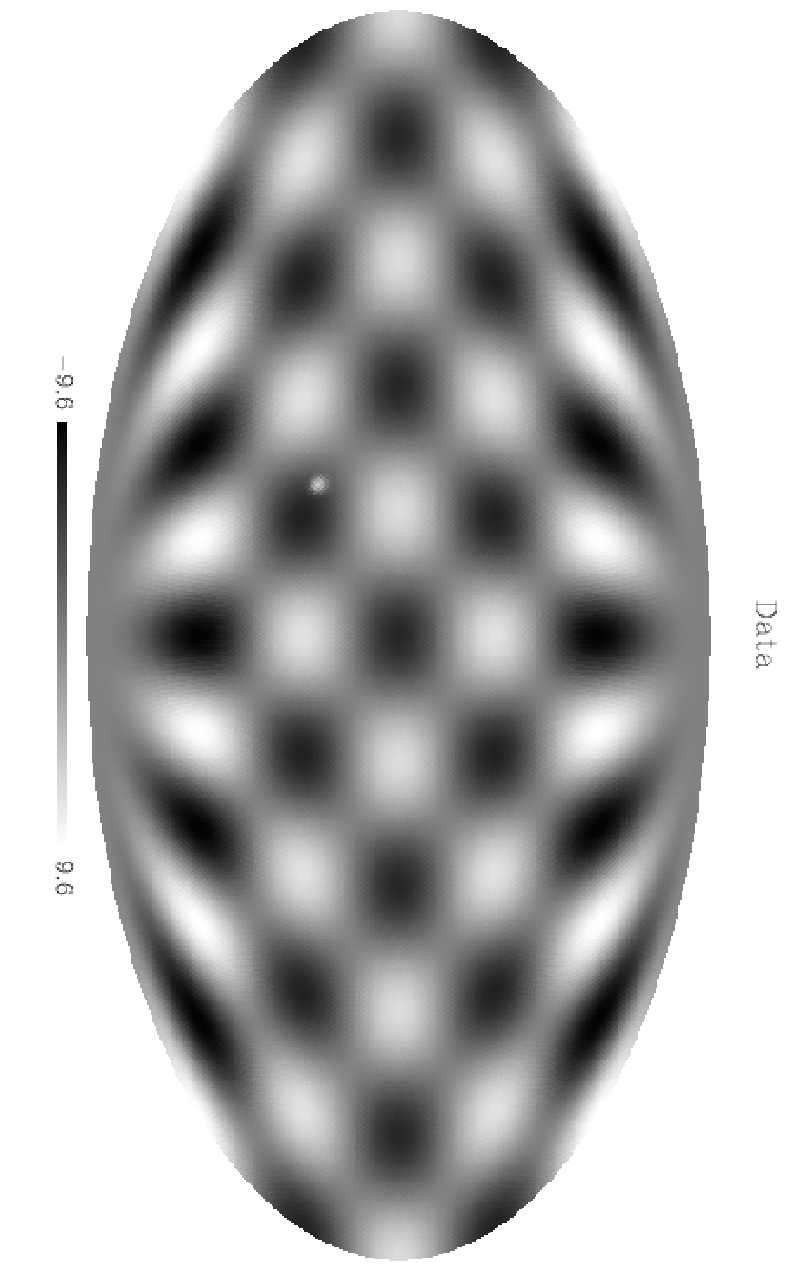
\includegraphics[width=6.5cm,height=4cm]{test_gauss_alm_bw.pdf}
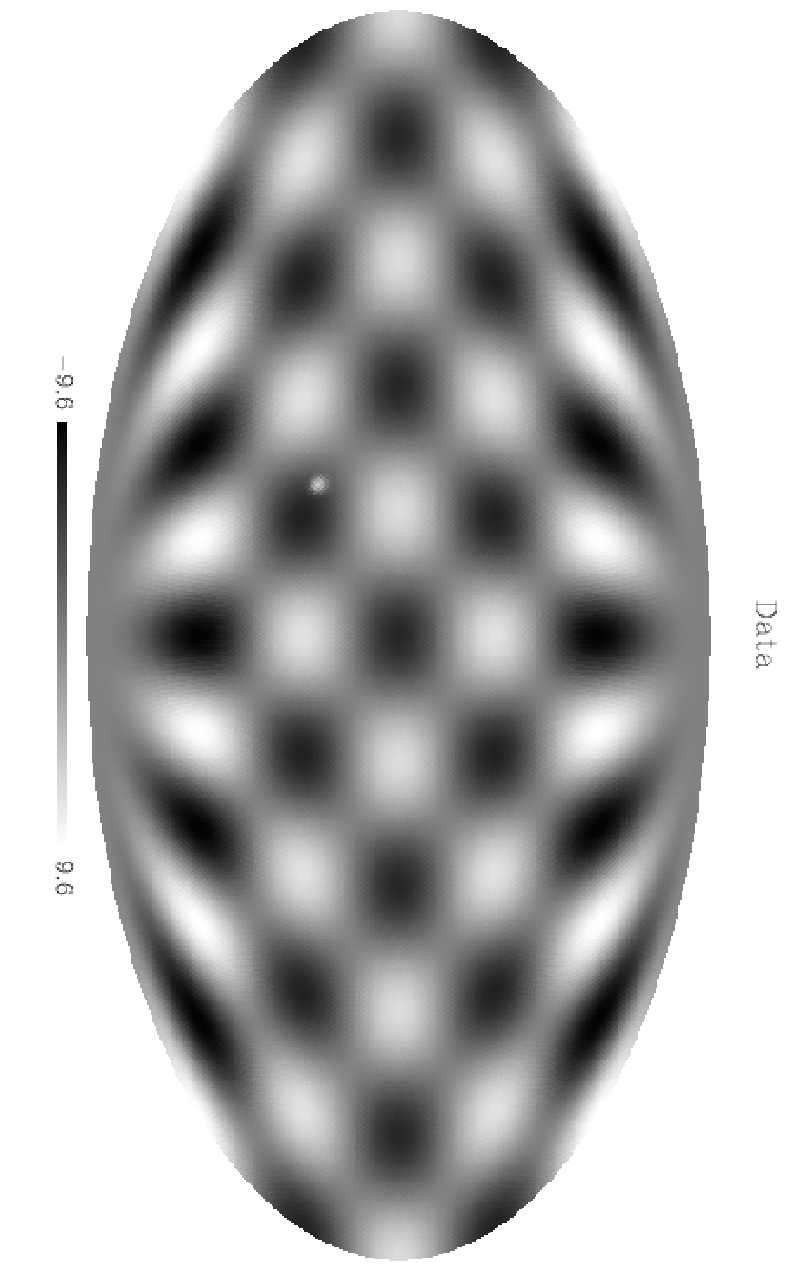
\includegraphics[angle=90,height=4.5cm,width=7.9cm]{test_gauss_alm_bw.pdf}
}}
\centerline{
\hbox{
% 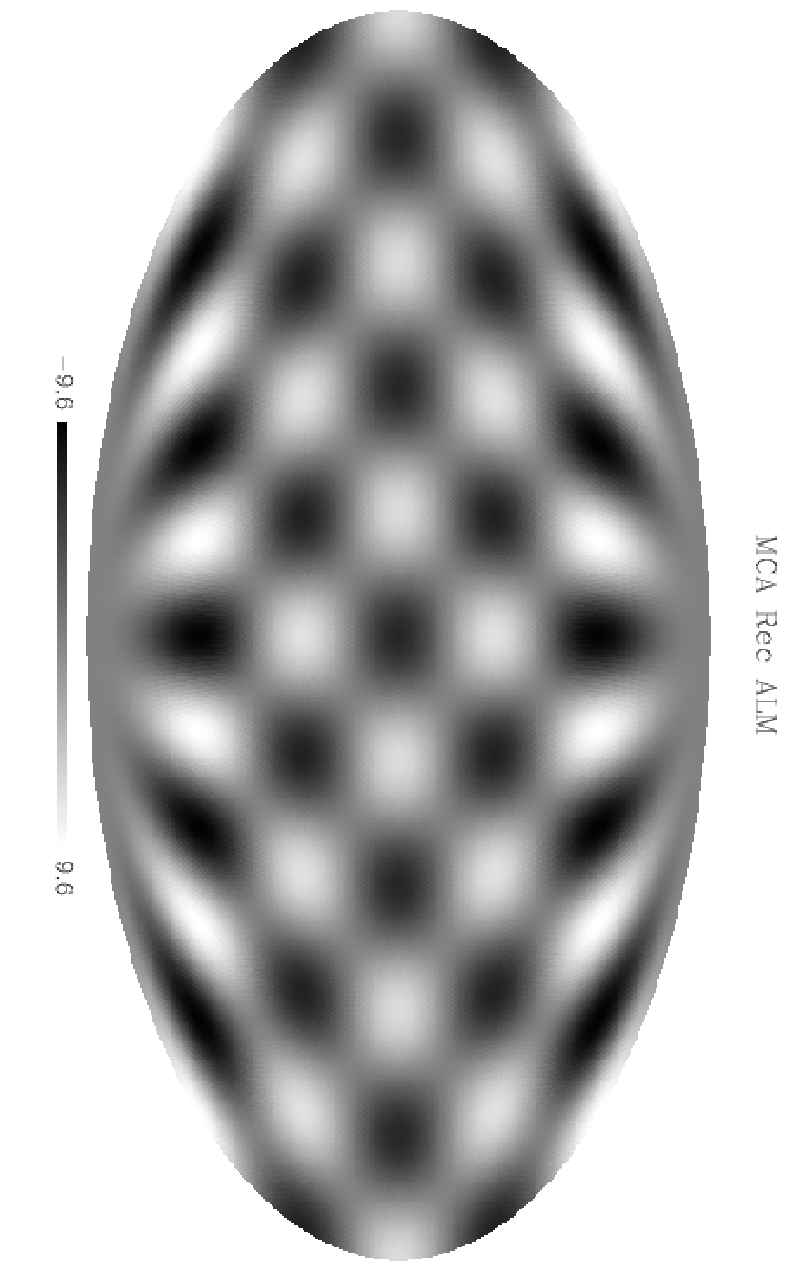
\includegraphics[width=6.5cm,height=4cm]{test_gauss_alm_mca_alm_bw.pdf}
% 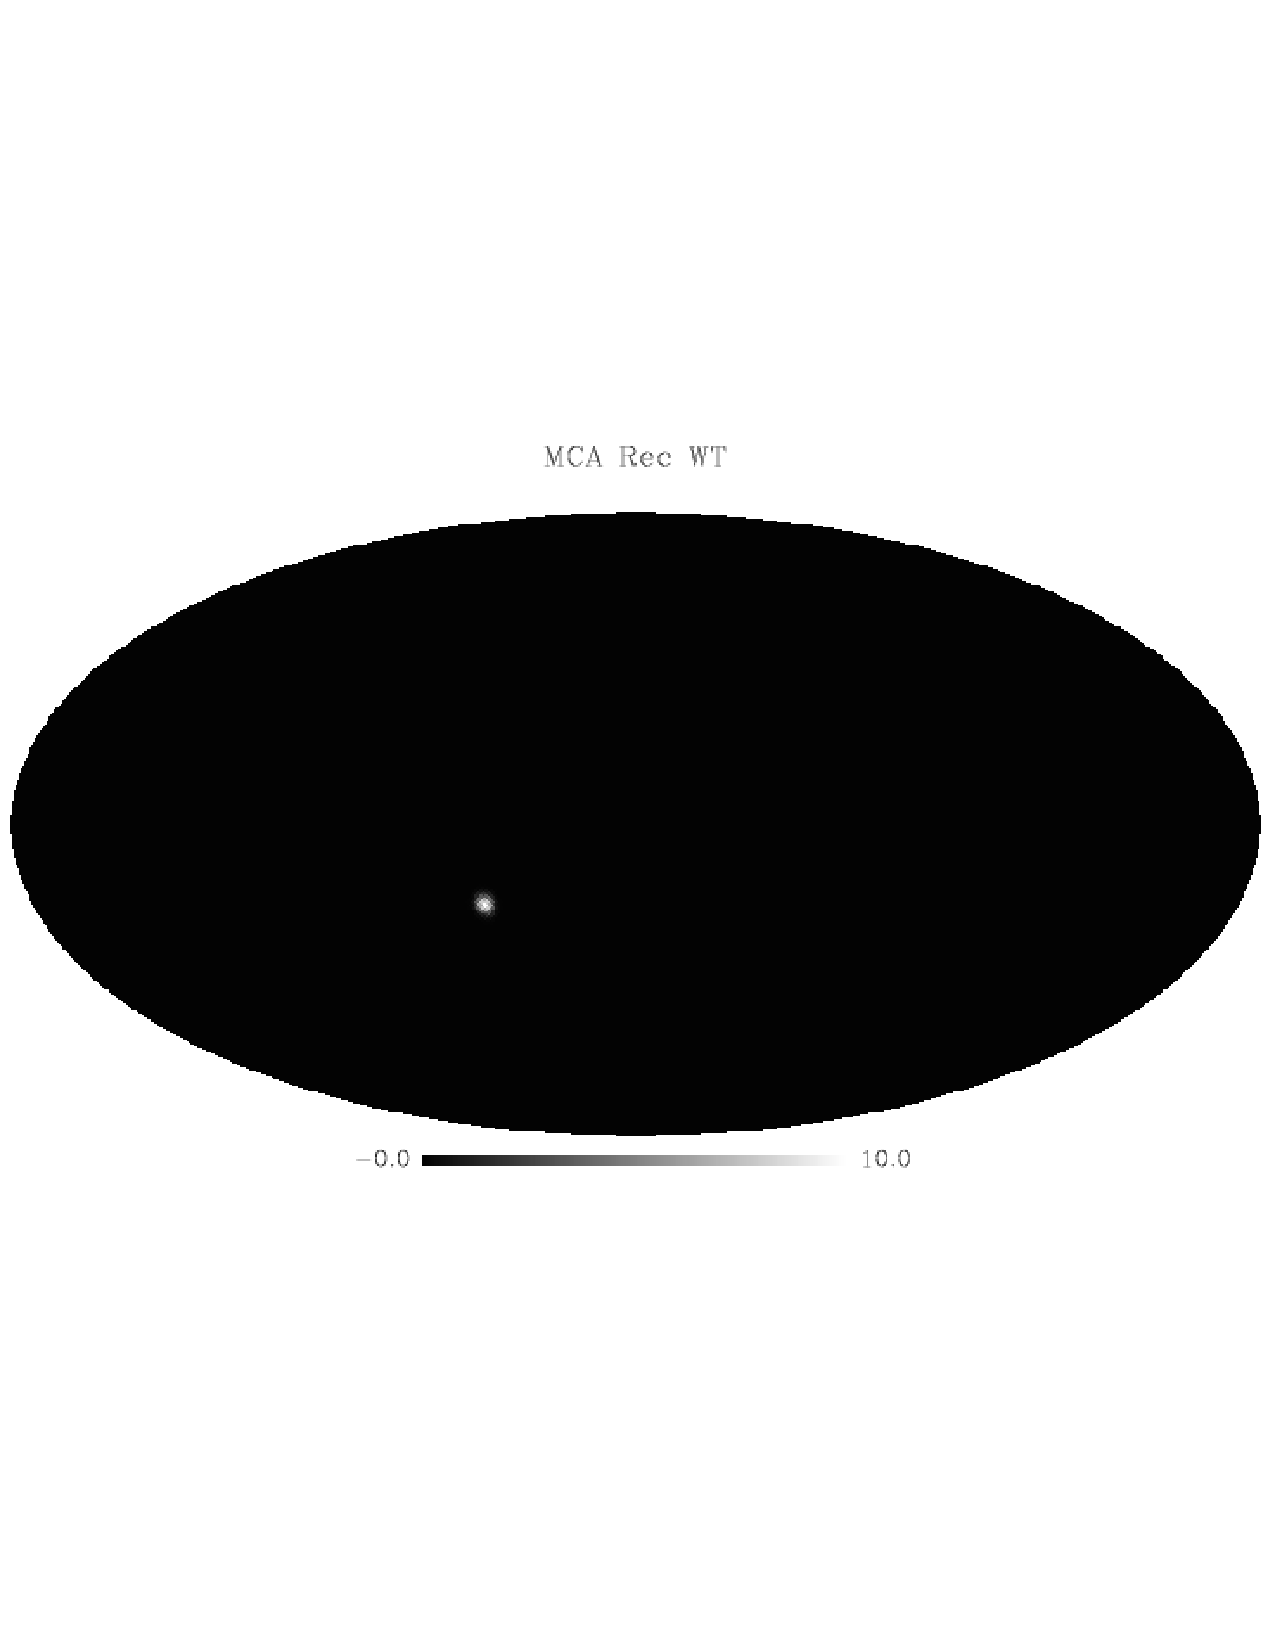
\includegraphics[width=6.5cm,height=4cm]{test_gauss_alm_mca_wt_bw.pdf}
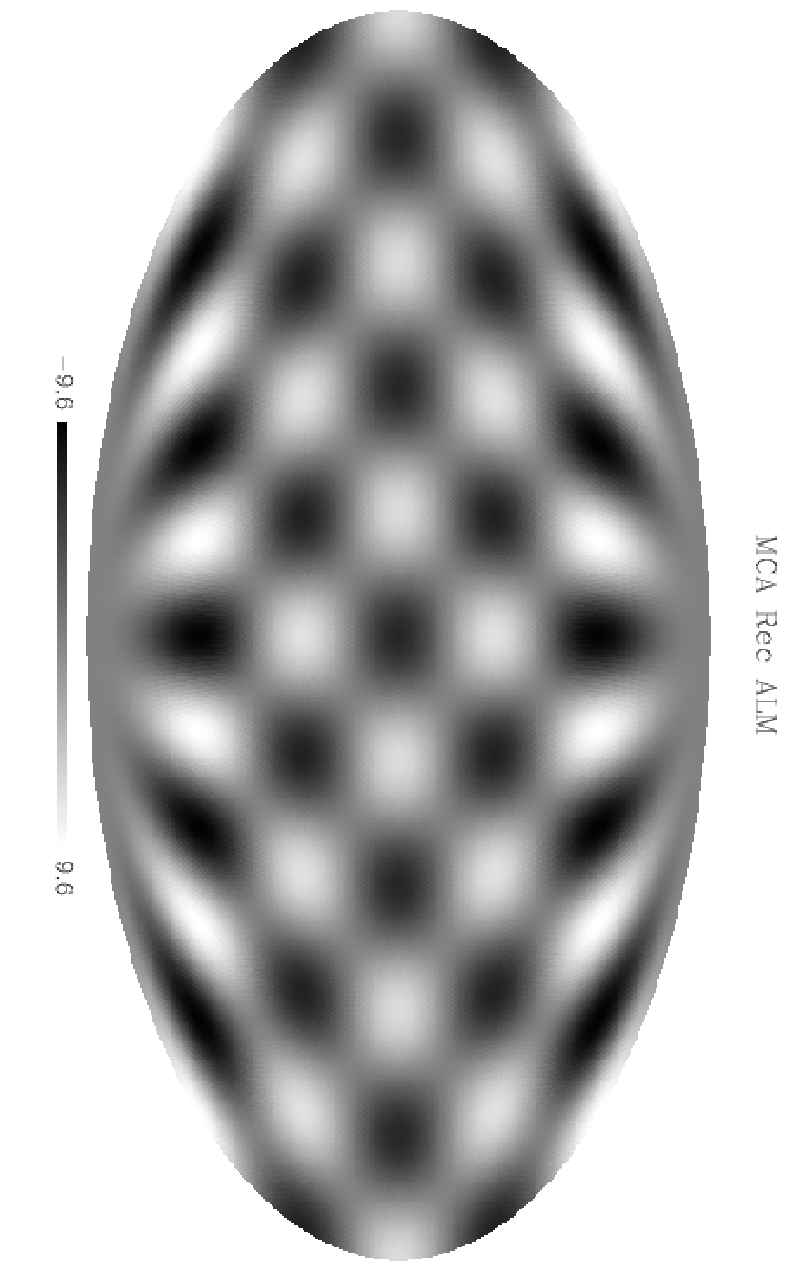
\includegraphics[angle=90,height=4.5cm,width=7.9cm]{test_gauss_alm_mca_alm_bw.pdf}
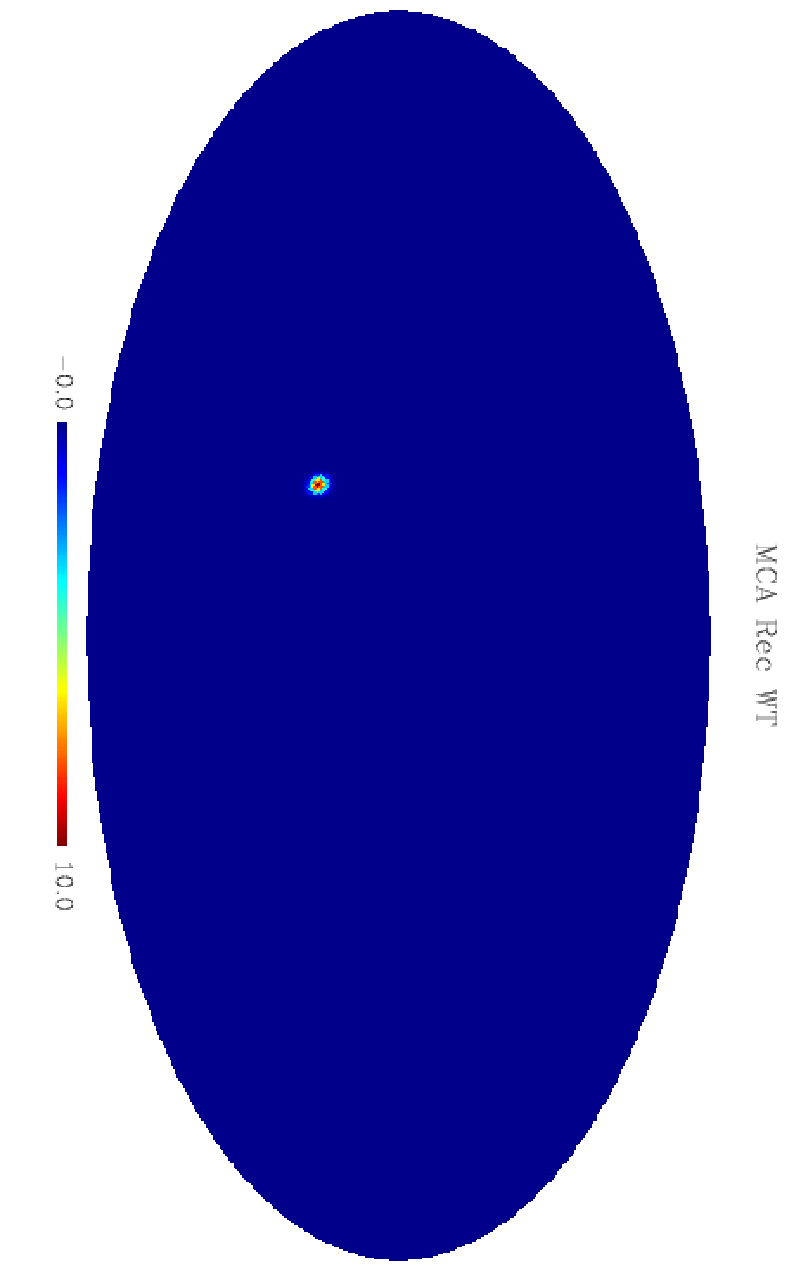
\includegraphics[angle=90,height=4.5cm,width=7.9cm]{test_gauss_alm_mca_wt.pdf}
}}
}
\caption{ Simple toy experiment with MCA on the sphere. 
The top map shows a linear combination of a spherical harmonic function 
and a localized Gaussian-like function on the sphere. The bottom maps 
show the resulting separated components that were obtained using the 
proposed Morphological Component Analysis on the sphere.}
\label{Figure:mcatoy}
\end{figure}
The spherical maps shown on { figure~\ref{Figure:mcatoy}} illustrate a simple numerical experiment. 
We applied the proposed Morphological Component Analysis on the Sphere to synthetic data resulting 
from the linear mixture of components respectively sparse in the spherical harmonics and the isotropic 
wavelet representations. The method was able to separate the data back into its original constituents. 
A more involved application is described in the next section.    
%---------------------------------------------------------------------------------------------------------------------------------------
\subsection{Application in Physics}
\label{section:bedros}
In Inertial Confinement Fusion (ICF) a spherical shell is irradiated by laser energy directly or after the 
laser energy has been converted to soft X-rays~\citep{bedros:atzeni}. Either way, the aim is to implode the 
capsule which contains a shell of nuclear fusion fuel (deuterium and tritium) ready to ignite if, after it 
has been imploded, its density is high enough and a hot spot in its center becomes hot enough to cause a 
propagating nuclear burn wave to travel through the rest of the fuel. This ultimate energy source will not 
work if during the implosion hydrodynamic instabilities develop which can break apart the shell before it 
assembles at the center and a hot spot forms~\citep{bedros:lindl}. Hydrodynamic instabilities such as Rayleigh-Taylor 
occur due to nonuniformities in the laser spatial profile or imperfections in the composition of multiple 
surfaces which make up the layers of thin material that surround the nuclear  fuel. Very small amplitude imperfections 
initially can result in the ultimate failure of the target due to the large compression ratios involved in ICF.
\begin{figure}
\centerline{
\hbox{
% \psfig{figure=bed_mca_orig_data.ps,bbllx=1.5cm,bblly=10cm,bburx=19cm,bbury=19.cm,height=4cm,width=6.5cm,clip=}
% \psfig{figure=bed_mca_large_scale.ps,bbllx=1.5cm,bblly=10cm,bburx=19cm,bbury=19.cm,height=4cm,width=6.5cm,clip=}
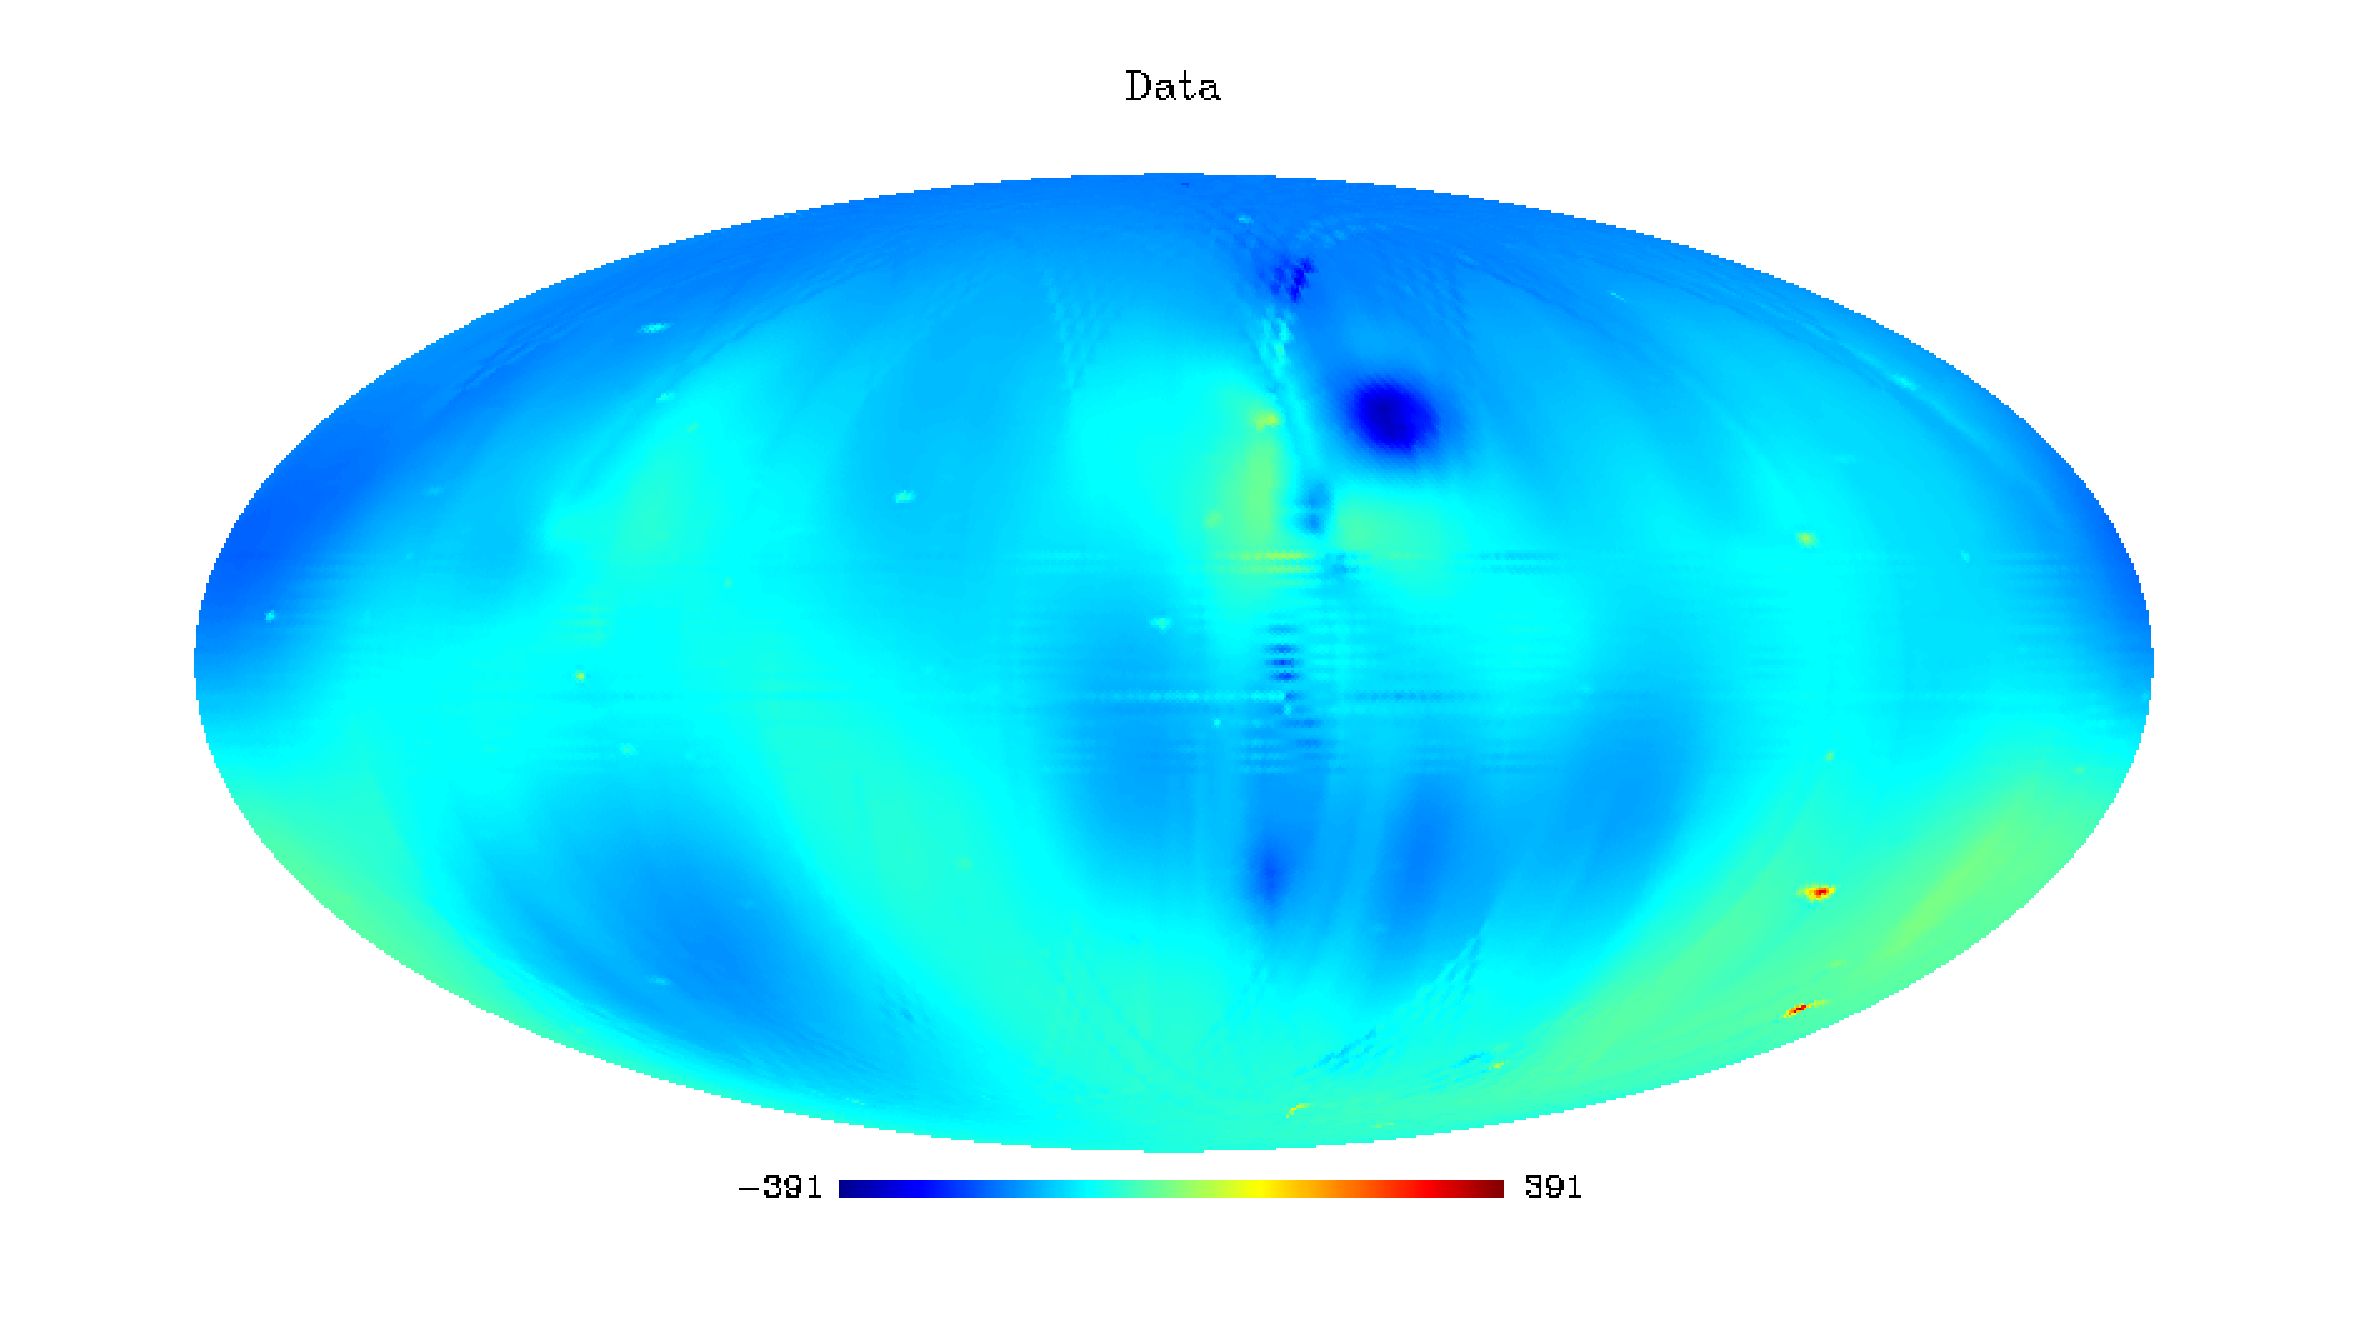
\includegraphics[angle=0,width=7.9cm]{bed_mca_orig_data.png}
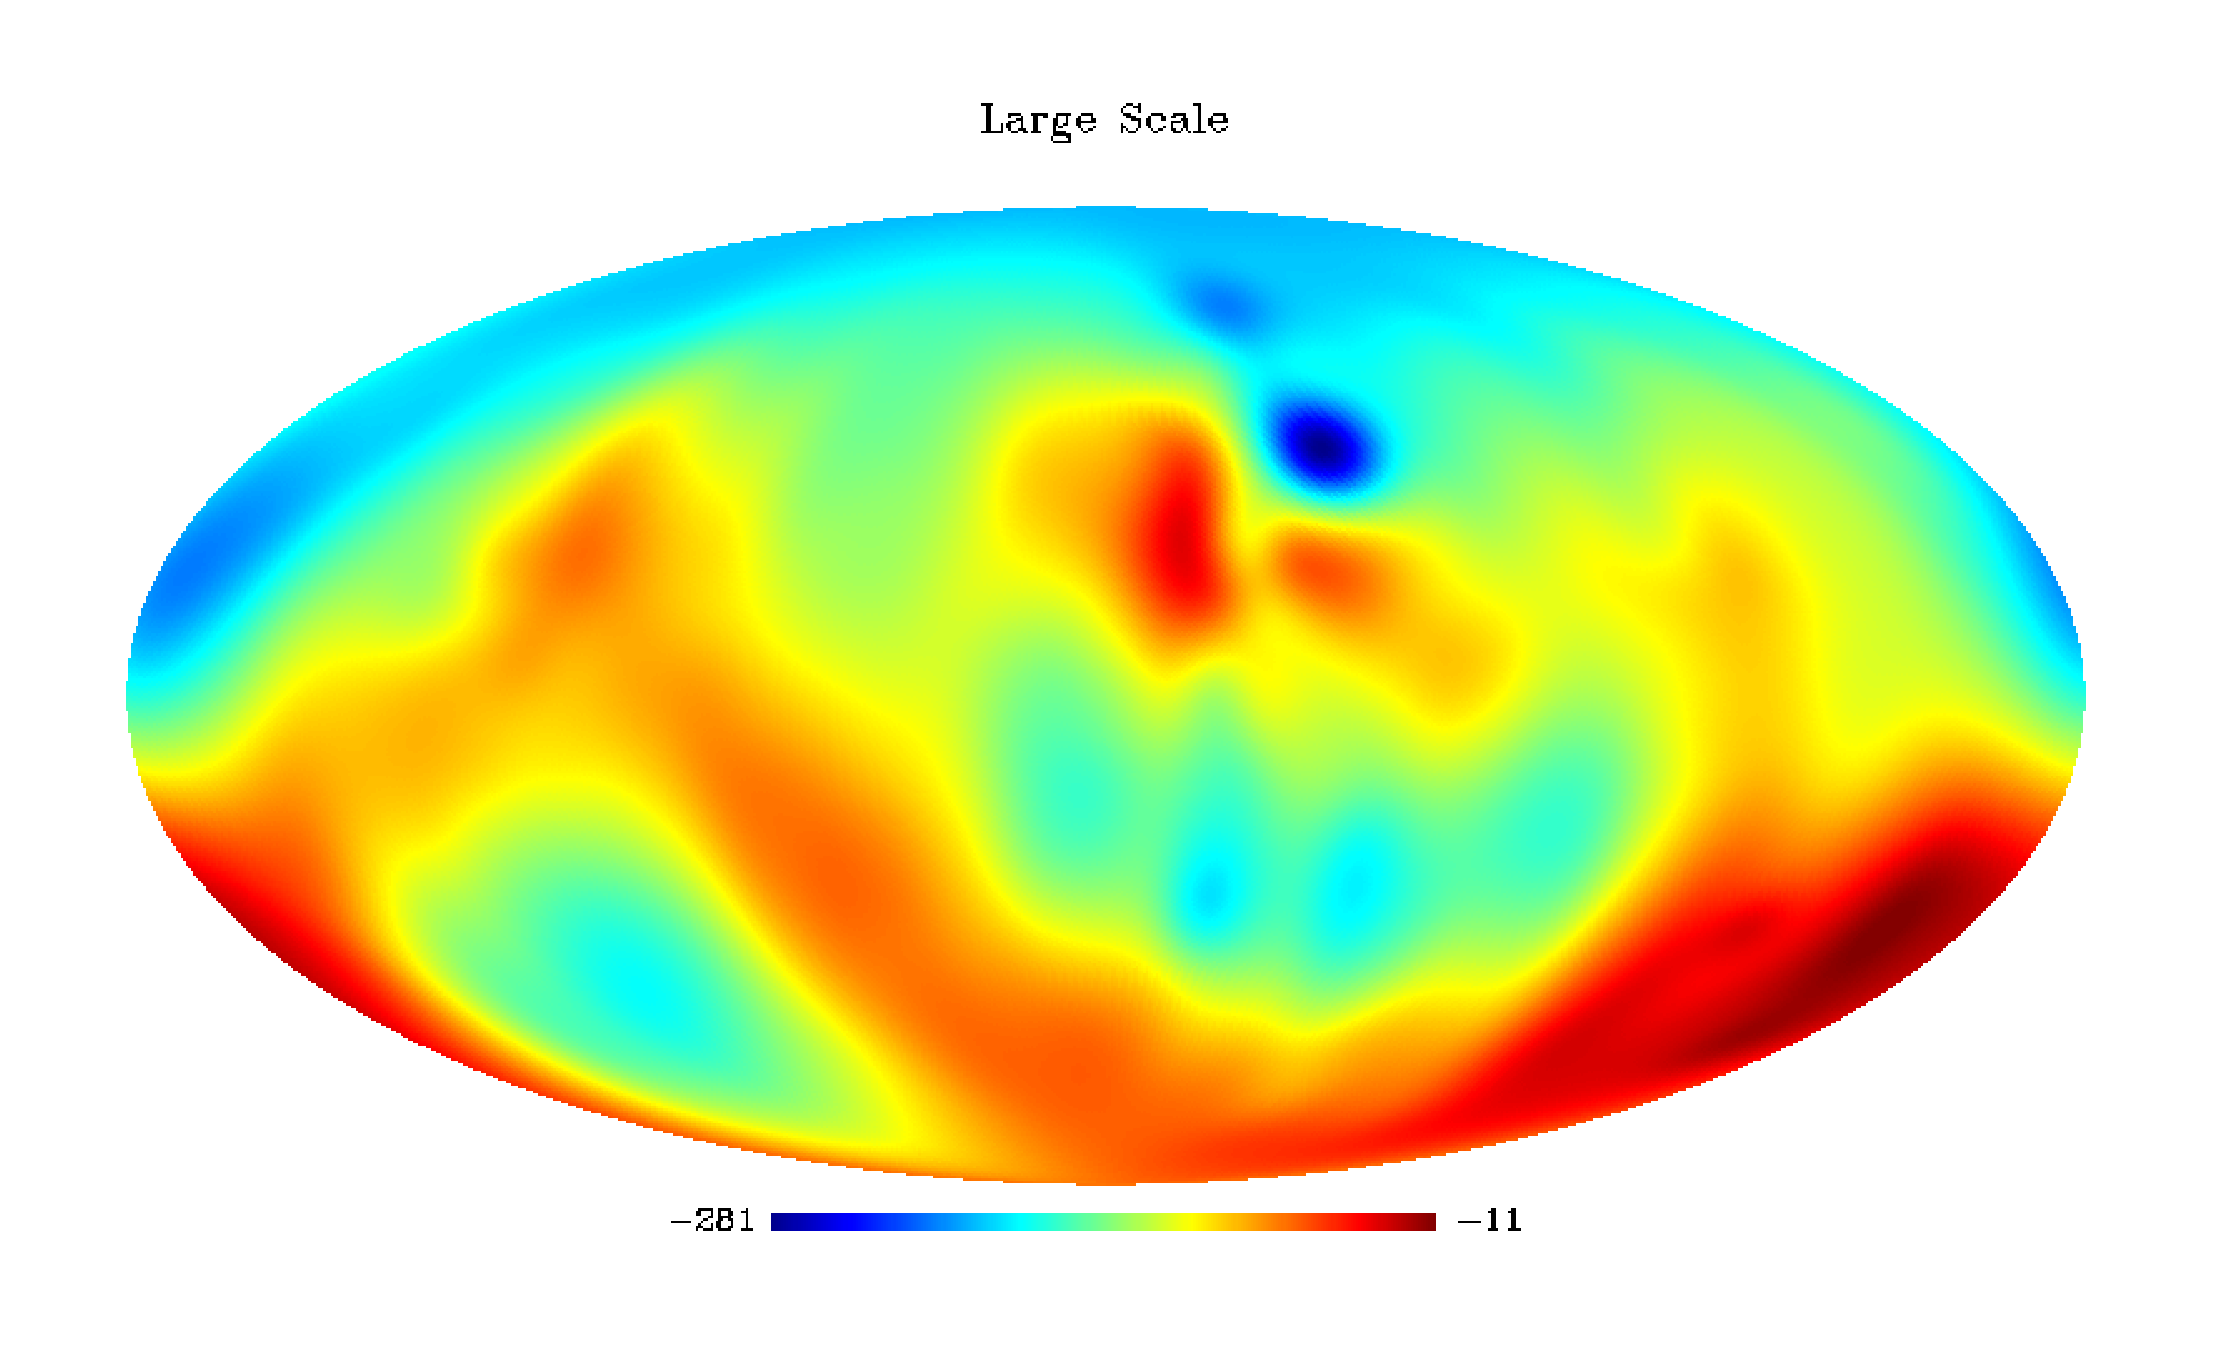
\includegraphics[angle=0,width=7.9cm]{bed_mca_large_scale.png}
}}
\caption{Left: Surface structures of ICF spherical shells measured on the nanometer scale are a superposition of global scale variations, isolated bumps and scratches as well as artifacts which look like interference patterns on intermediate scales. Right: Coarsest scale of the undecimated isotropic wavelet transform of the surface measurements of an ICF target.}
\label{bedros_mca_data}
\index{data!plasma confinement}
\end{figure}
It is therefore extremely important to characterize the inner and outer surfaces of ICF shell targets 
so as to know whether they are worthy of consideration for ICF implosions. One day in a reactor setting 
tens of thousands of targets will have to be imploded daily so that checking each one is totally 
out of the question. Instead, very good target fabrication quality control processes have to be adopted so that 
confidence levels in proper performance will be high. A major step along this path to fusion energy then is to 
understand why imperfections occur and to correct the systematic elements and control the harm done by random sources.
%
Fine structures on the surfaces of spherical shells can be measured on the nanometer scale, among others, 
by atomic force microscopy or phase shifting spherical diffractive optical interferometry. An example of 
such measurements is shown on figure~\ref{bedros_mca_data}. As can be seen from the figure, there appears 
to be a superposition of global scale variations, isolated bumps and scratches as well as artifacts which 
look like interference patterns on intermediate scales of localization. The latter must be isolated and 
eliminated from consideration when deciding the readiness of the target for implosion. We have achieved 
the morphological feature separation by first doing an isotropic wavelet transform on the spherical data 
and subtracting the coarsest scale information. MCA on the sphere was used on the rest of the image using 
the undecimated wavelet and the local cosine transforms on the sphere. The isolated bumps were thus identified 
and the measurement technique caused artifacts were removed easily. The resulting bumps added to the coarsest scale, 
is the clean data with the interference patterns and artifacts removed as shown in figure~\ref{bedros_mca_result}. 
The spherical harmonic decomposition of the cleaned image gives rise to coefficients of various $\ell$ modes 
which will be amplified by the implosion process which can now be assessed correctly using numerical hydrodynamics 
simulation generated growth factors. If the bumps are clustered and not randomly distributed, then systematic errors 
in the manufacturing process can be tracked down. A code called MODEM has been put together to study such 
target surface data and extract the localized bump statistics including their correlations in height, 
size and relative location. For more details see~\citep{bedros:modem}.
\begin{figure}[htb]
\centerline{
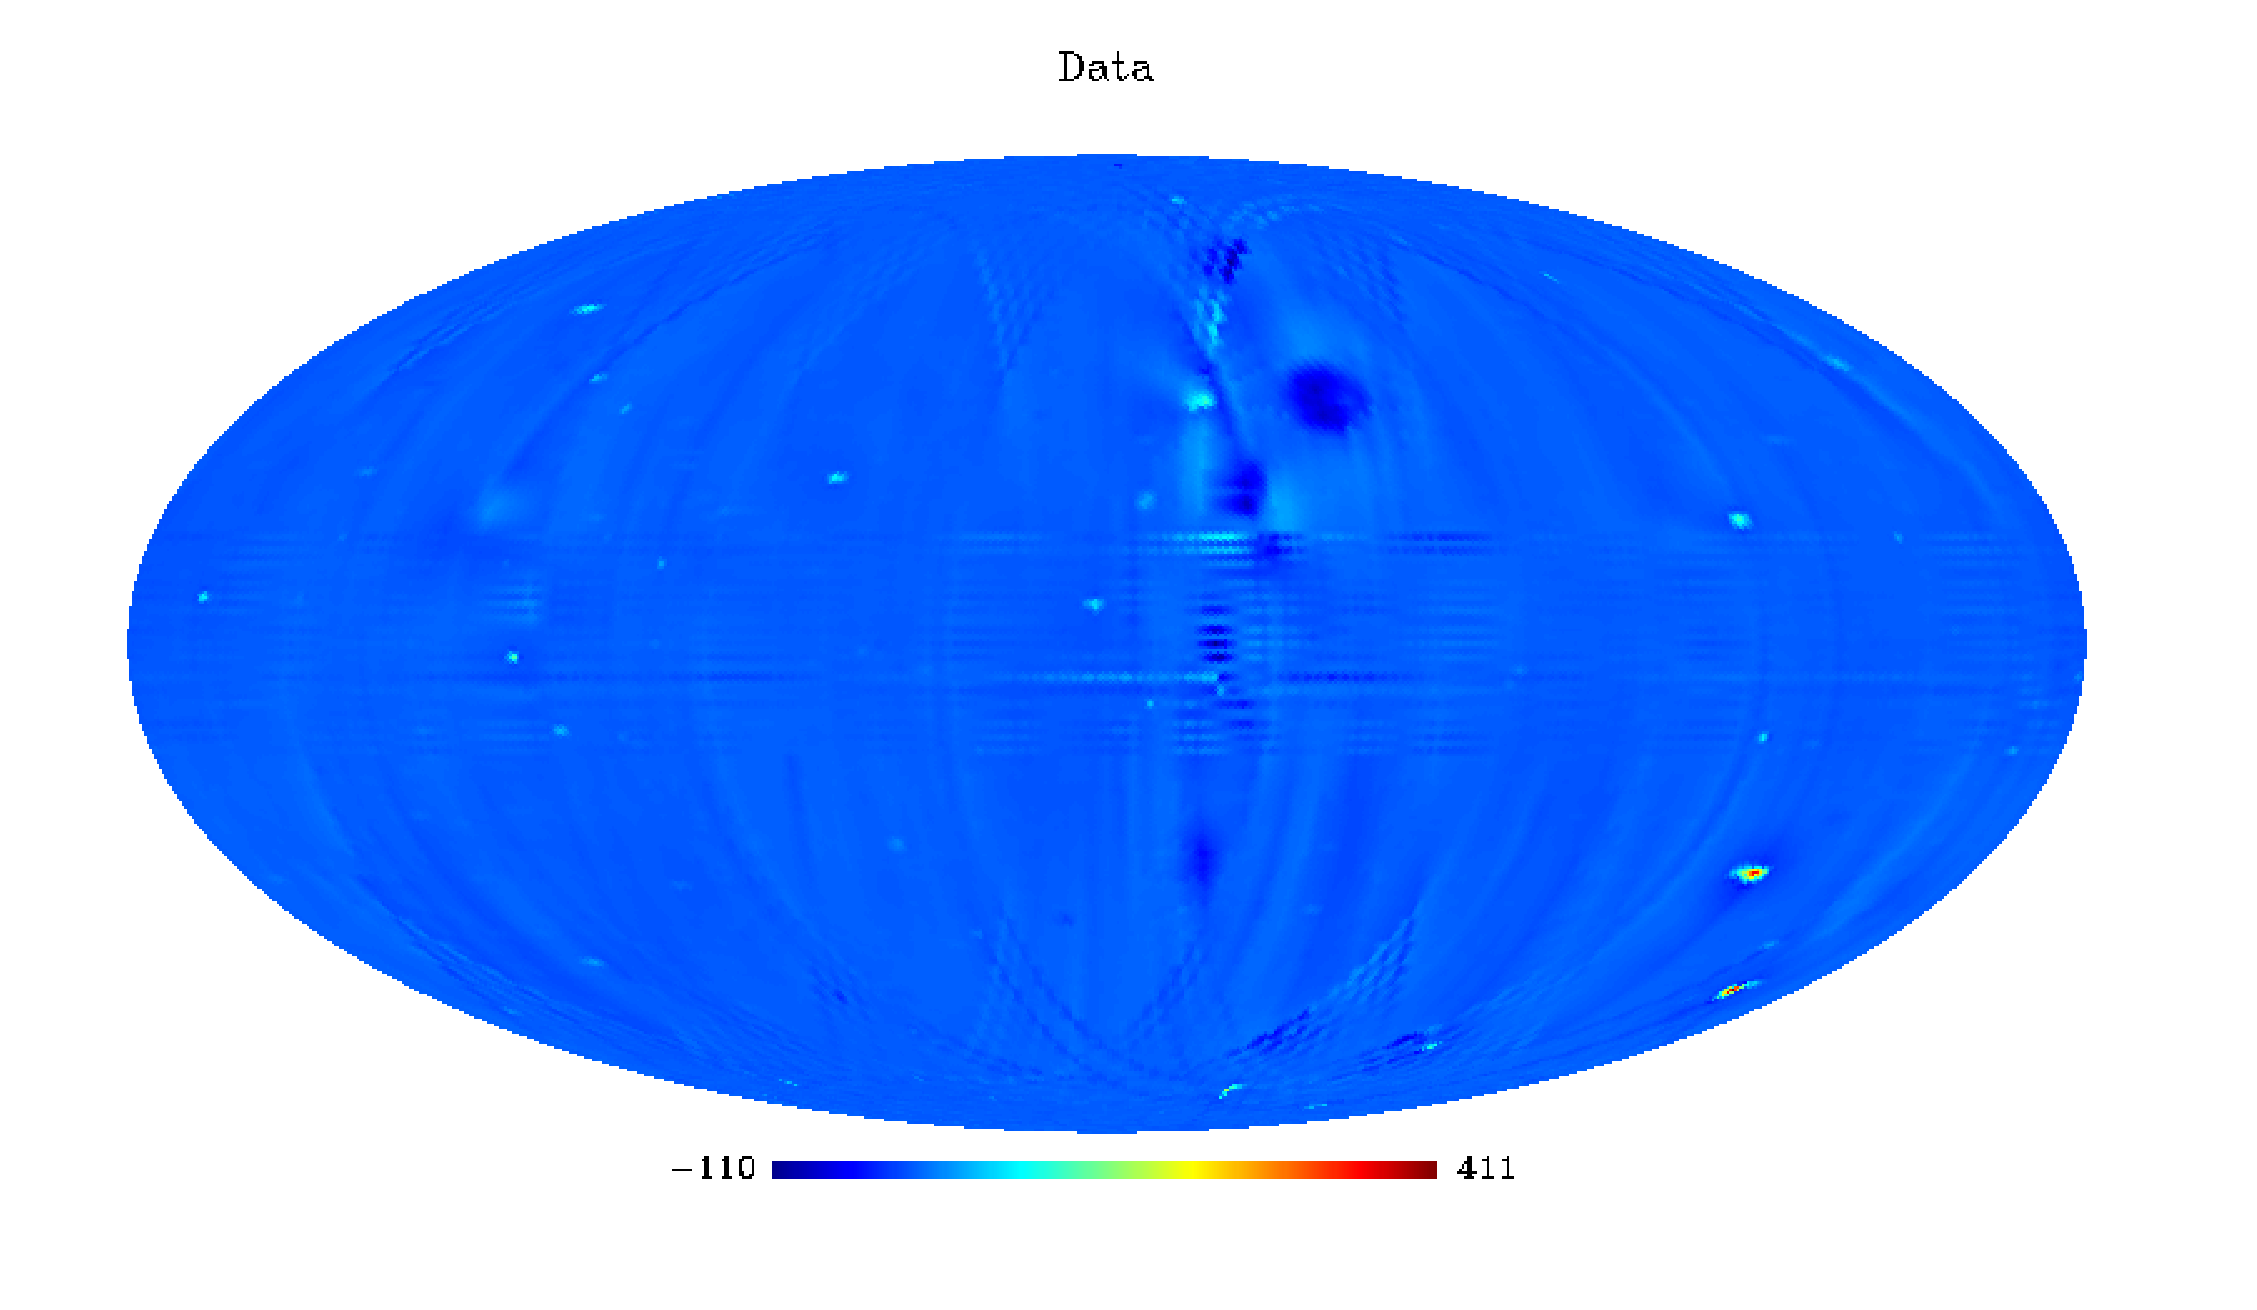
\includegraphics[angle=0,width=7.9cm]{bed_mca_in_data.png}
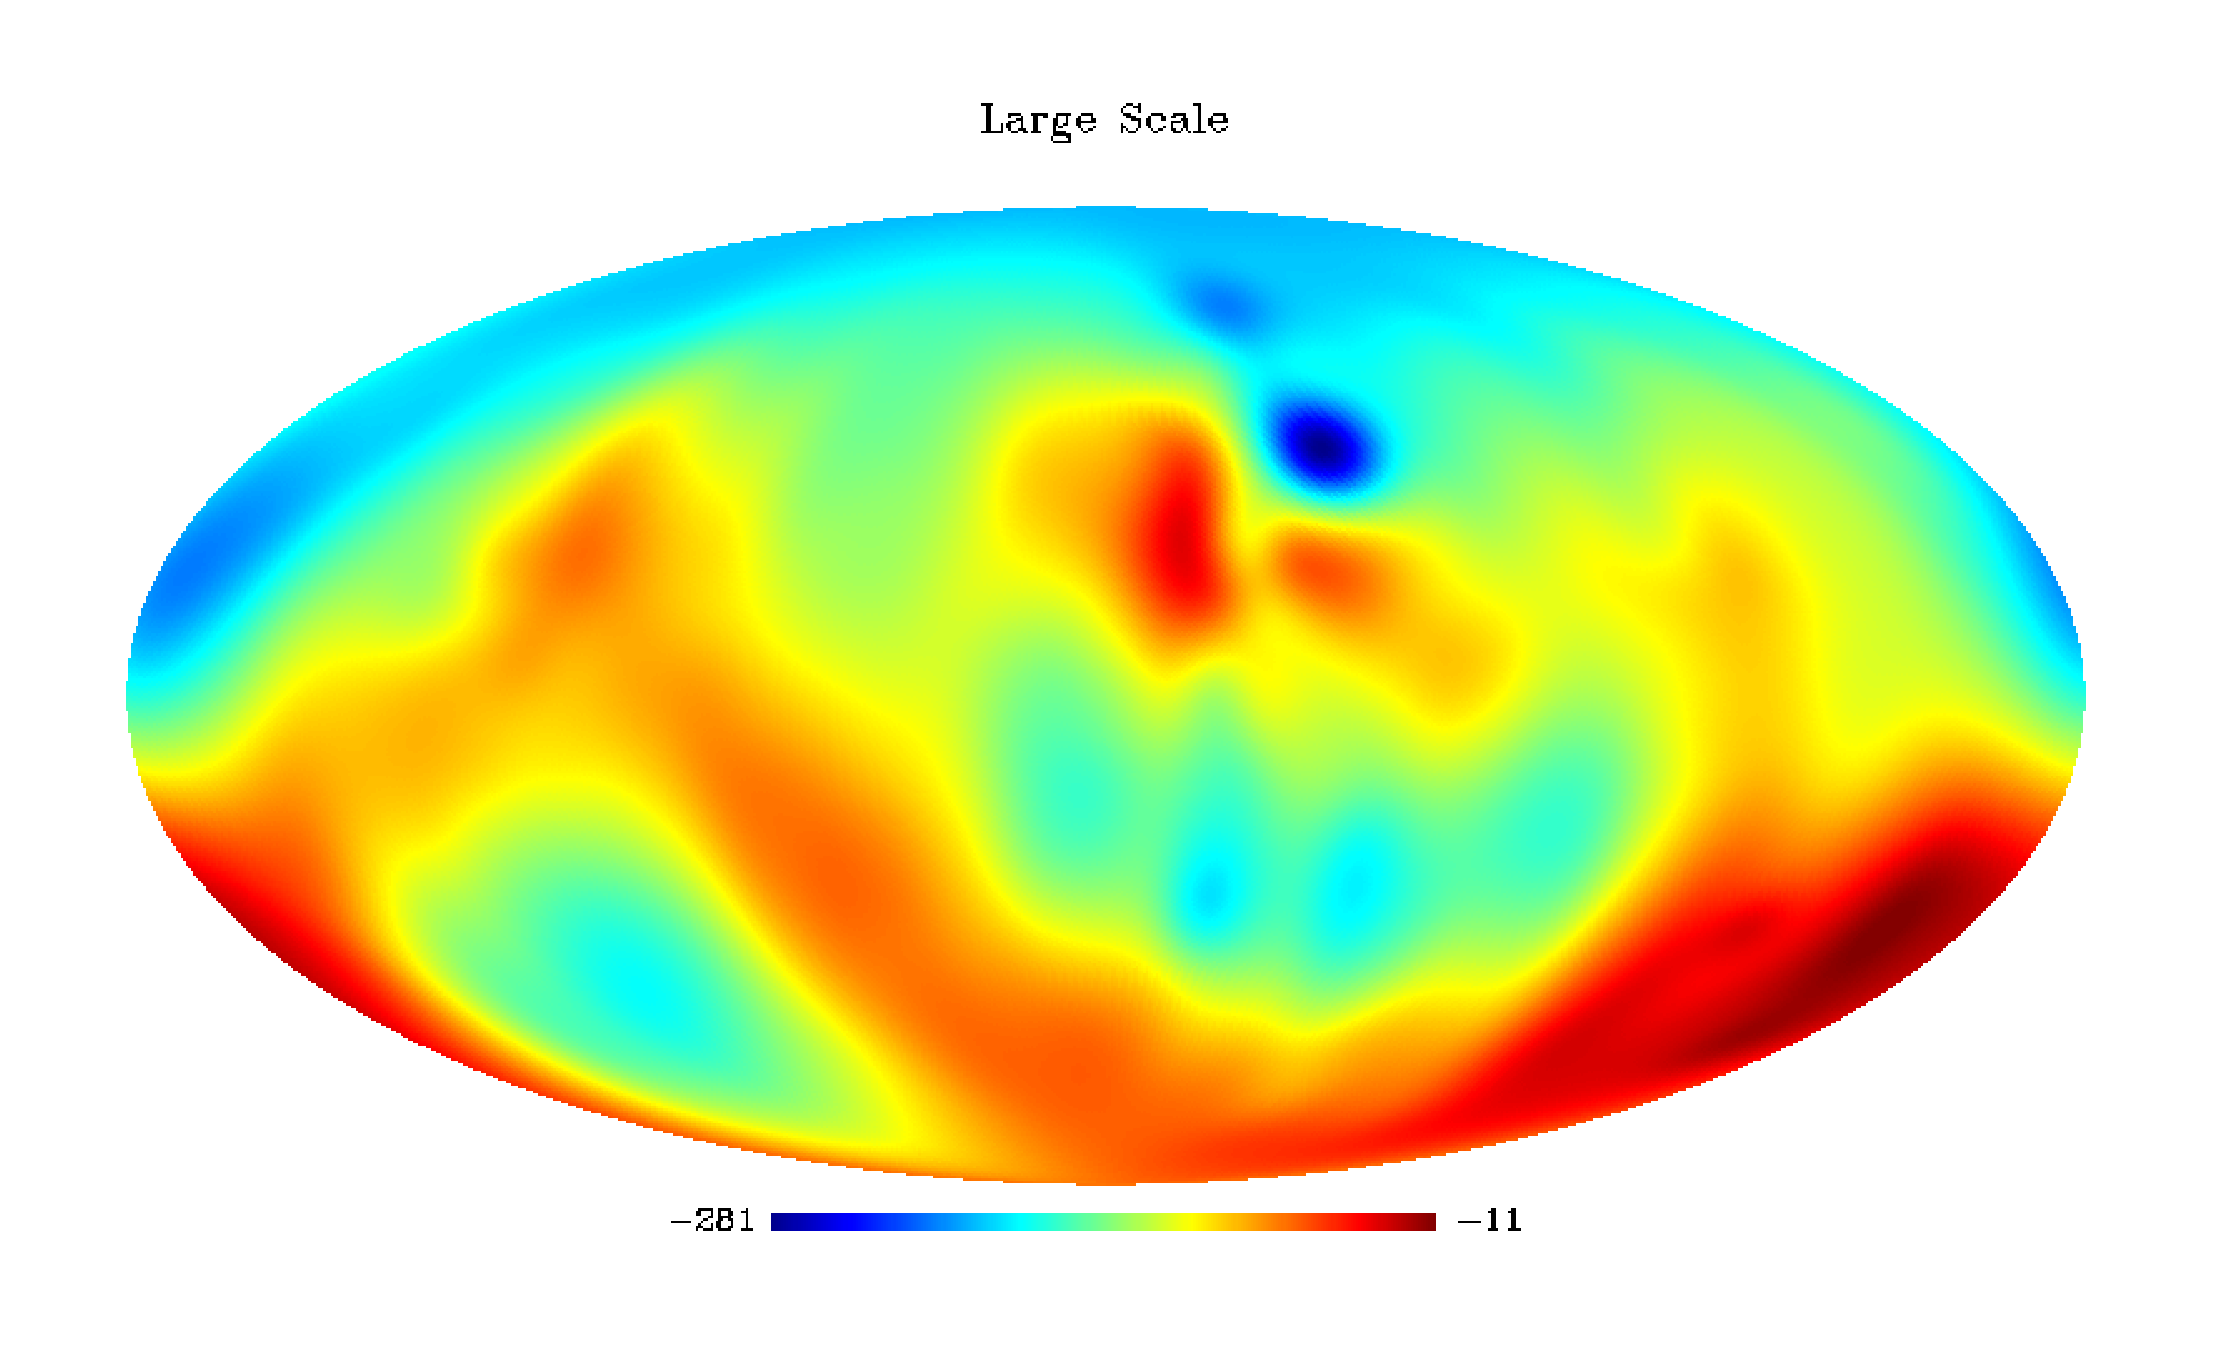
\includegraphics[angle=0,width=7.9cm]{bed_mca_large_scale.png}
}
\centerline{
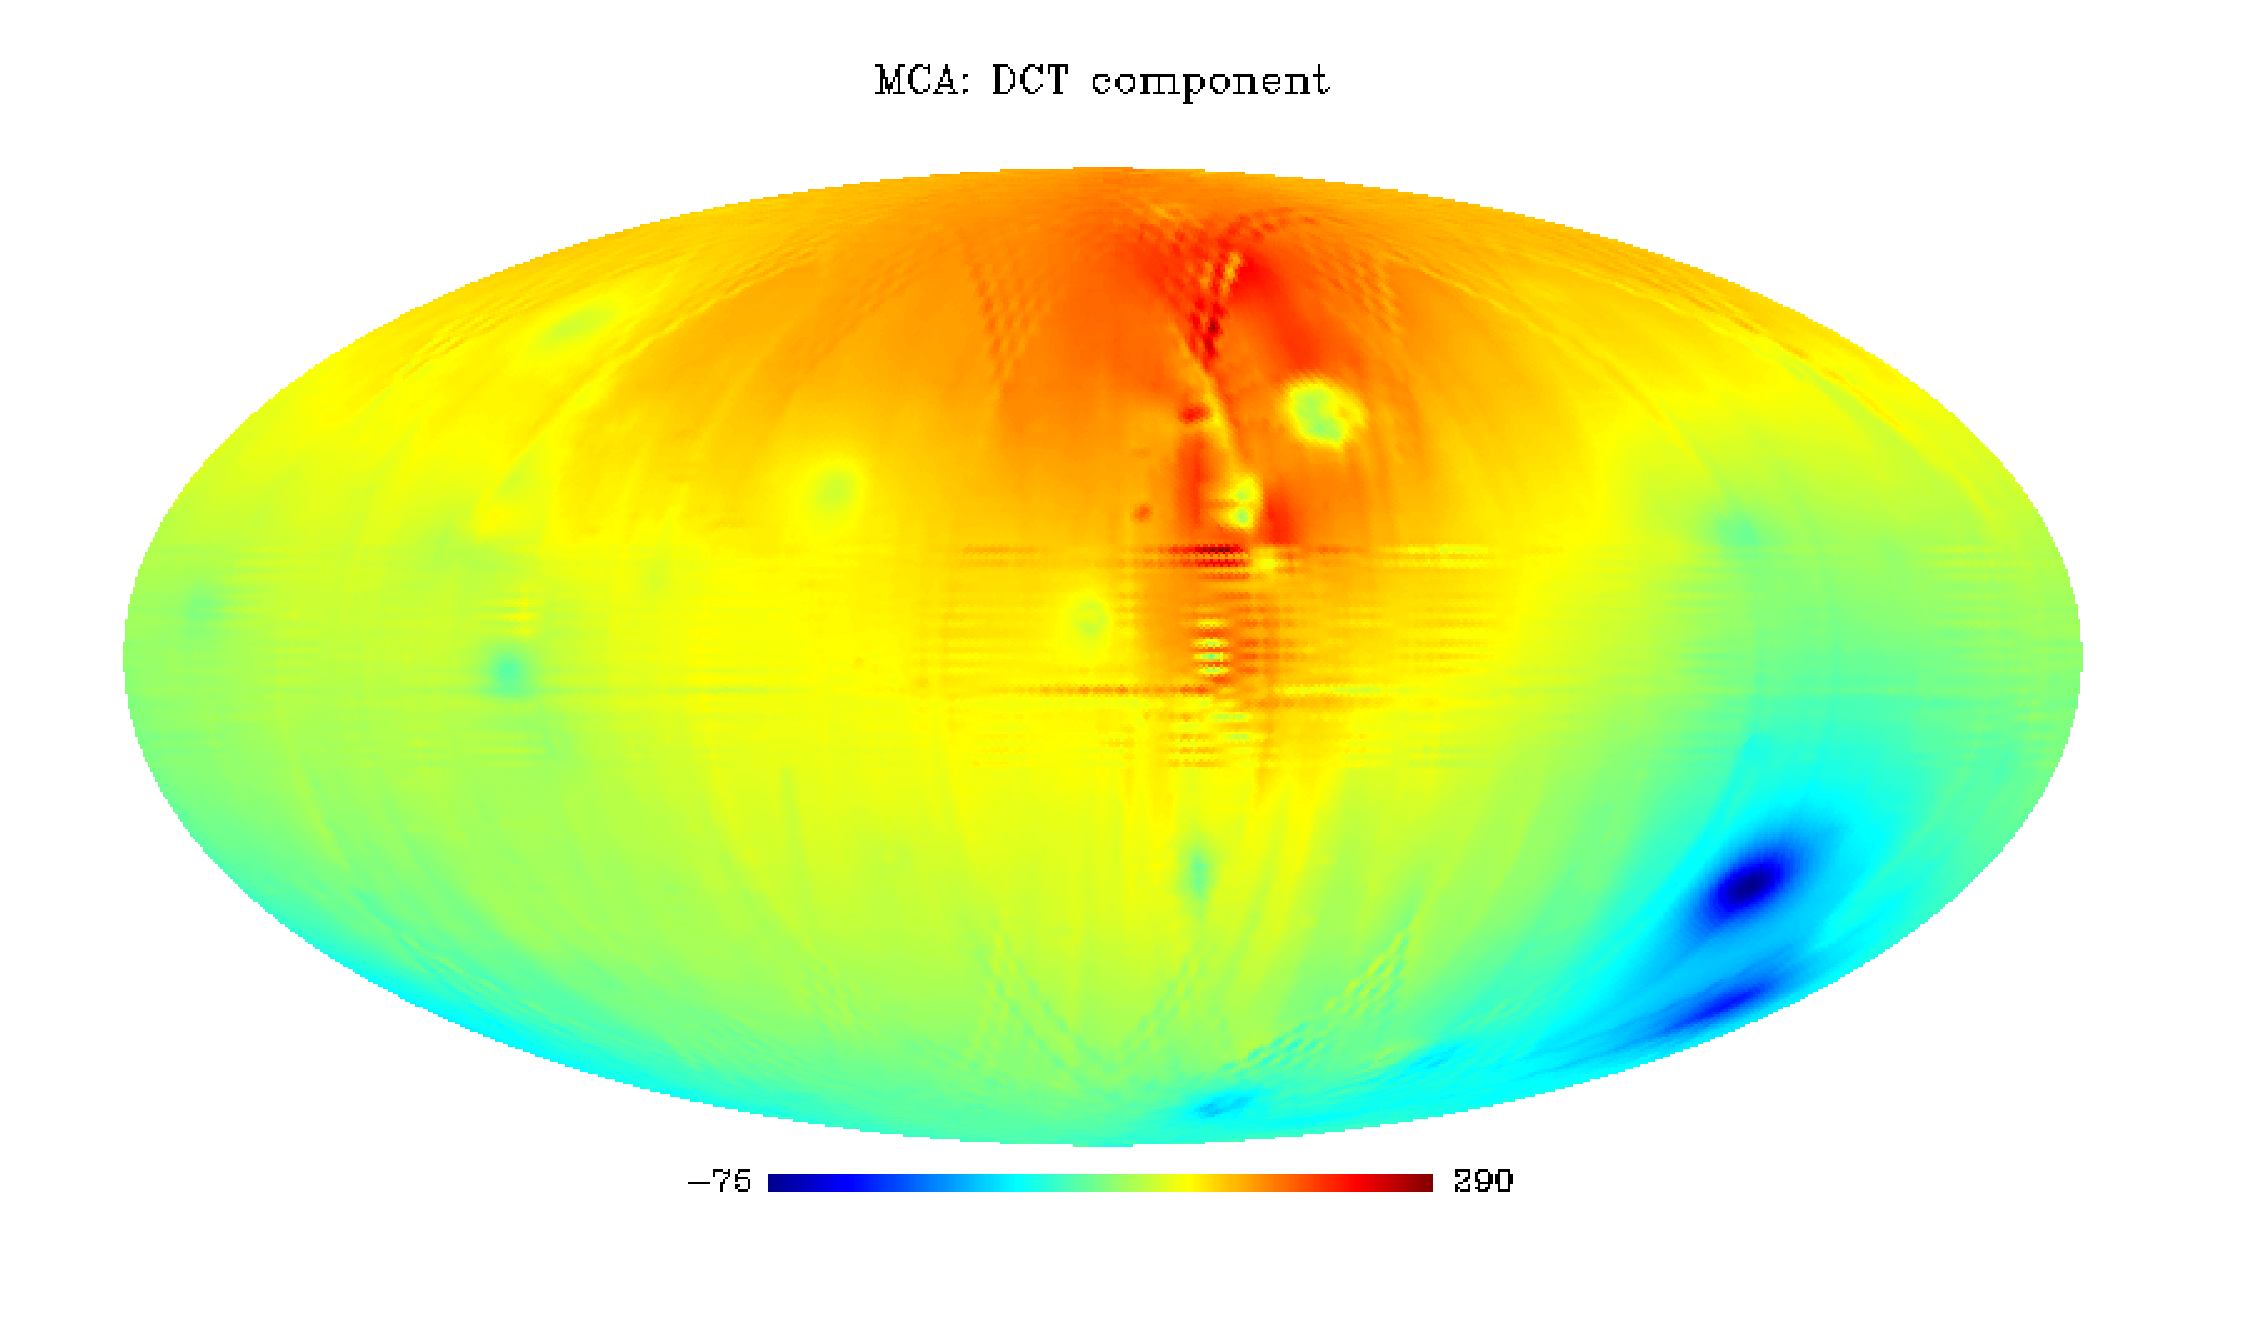
\includegraphics[angle=0,width=7.9cm]{bed_mca_out_dct.png}
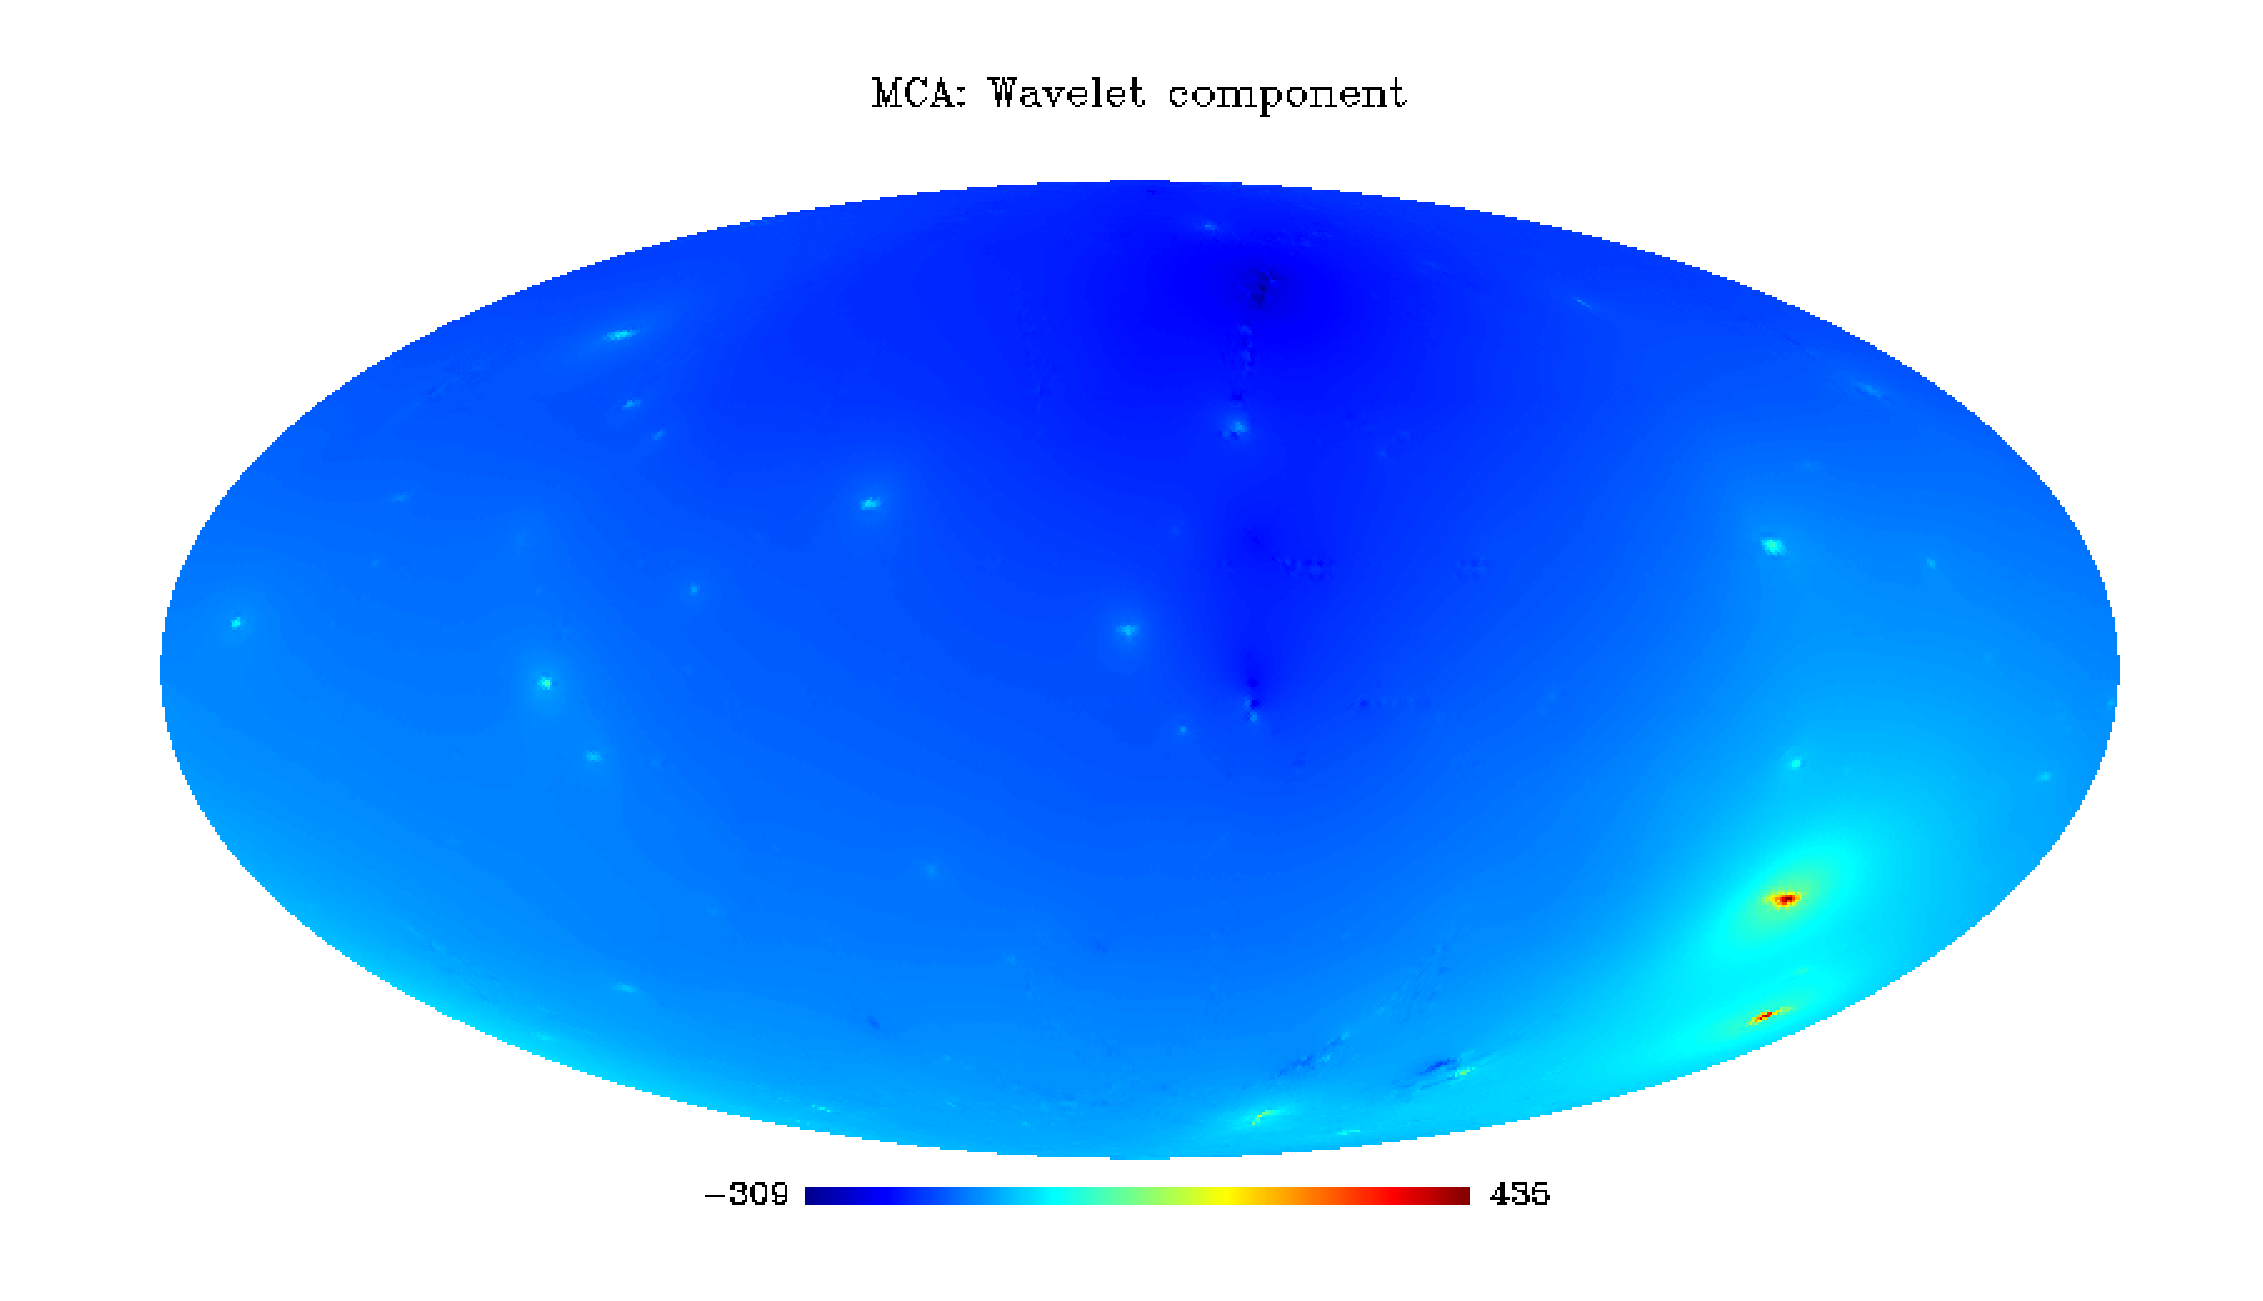
\includegraphics[angle=0,width=7.9cm]{bed_mca_out_wt.png}
}
\caption{Top: Spherical map obtained by subtracting the coarse scale map on the right of Fig.~\ref{bedros_mca_data} from the initial map on the left of Fig.~\ref{bedros_mca_data}. Bottom: Component maps separated by the MCA method on the sphere: interference patterns and measurement artifacts were caught by the local cosine functions on the sphere (left) while  the isolated bumps were caught using the undecimated wavelet on the sphere (right). Adding back the coarse scale on the right of Fig.~\ref{bedros_mca_data} to the latter map results in a clean map of the surface structures of an ICF spherical shell with the interference patterns and artifacts removed.} 
\label{bedros_mca_result}
\index{data!plasma confinement}
\end{figure}
%---------------------------------------------------------------------------------------------------------------------------------------
\section{Inpainting on the Sphere}
\label{sect_inpaint}
%---------------------------------------------------------------------------------------------------------------------------------------
\subsection{Algorithm}
%---------------------------------------------------------------------------------------------------------------------------------------
Named after the expert recovery process used for the restoration of deteriorated masterpieces, inpainting refers to a set 
of techniques used to alter images in a way that is undetectable to people who are unaware of the original images. There are 
numerous applications among which removing scratches or objects in digitized photographs, removing overlayed text or graphics, 
filling-in missing blocks in unreliably transmitted images, predicting values in images for better compression or image upsampling. 
Inpainting algorithms strive to interpolate through the gaps in the image relying on the available pixels, the continuation of edges, 
the periodicity of textures, etc. The preservation of edges and texture, in other words discontinuities, across gaps has attracted 
much interest, and many contributions have been proposed to solve this interpolation task. Non-texture image inpainting has received 
considerable interest and excitement since the pioneering paper by Masnou and Morel \citep{Masnou98, Masnou02} who proposed variational 
principles for image disocclusion. A recent wave of interest in inpainting has started from the recent contributions of Sapiro 
and al.~\citep{text:sapiro1,text:sapiro2,text:sapiro3}, followed by Chan and Shen~\citep{text:chan1}. In these works, authors point 
to the importance of geometry and design anisotropic diffusion PDEs to fill in gaps by smooth continuation of isophotes. 
PDE methods have been shown to perform well on piecewise smooth functions.
% 
A very different approach is the inpainting algorithm based on MCA described in~\citep{starck:elad05} which has proved capable 
of filling in holes in either texture or cartoon content in 2D images. To make the link between building sparse representations 
and inpainting, consider the effect of a rectangular gap on the set of Fourier coefficients of a monochromatic sinewave : 
because of the non-locality of the Fourier basis functions it takes a large number of coefficients to account for the gap, 
which is known as the Gibbs effect. Seeking a sparse representation of the incomplete sine-wave outside the gap, that is without 
fitting the gap, enables the recovery of the complete monochromatic sinewave.
%
Following~\citep{starck:elad05}, an inpainting algorithm on the sphere is readily built from the Morphological Component Analysis 
on the sphere described in the previous section. Consider a discrete spherical data map $y$ and a binary map $M$ such that ones 
in $M$ indicate that the corresponding pixels in $y$ are valid data while zeros indicate invalid data. The objective function of 
MCA~equation~\eqref{mca:model1} can be modified as follows : 
 \begin{equation}\label{inp:model}
\min_{s_1,\ldots,s_n} \lambda \sum_{k=1}^K  \|\alpha_k\|_1 + \left\|M  \odot (y-\sum_{k=1}^K s_k) \right\|_2^2\,\,\,\textrm{with}\,\,\,s_k ={\bf \Phi}_k \alpha_k .
\end{equation}
where $\odot$ stands for entry-wise multiplication. Thus we are preventing the sparse model under construction from attempting to fit 
the invalid data. Other constraints can be easily imposed on the interpolated sparse components. For instance, in~\citep{starck:elad05}, 
a total variation penalty is shown to enhance the recovery of piece-wise smooth components. Asking for the regularity across the gaps of 
some localized statistics (~e.g. enforcing that the empirical variance of a given inpainted sparse component be nearly equal 
outside and inside the masked areas) are other possible constraints. In practice, because of the lack of accuracy of some digital 
transformations we used in the spherical topology, additional constraints, which may be relaxed close to convergence, were also found 
useful in some cases to stabilize the described iterative algorithms. 
%
It is proposed that a solution to the above minimization problem can be reached using the same iterative thresholding process as 
in the MCA algorithm detailed in the previous section, with the only required modification consisting in masking the full 
residual using $M$ after each residual estimation, thus giving the MCA-inpainting algorithm~\ref{algo_mca_inp}.

%\begin{center}
%\begin{minipage}[b]{0.9\linewidth}
%\vspace{0.1in}
%\footnotesize{\textsf{1. Set the number of iterations $I_{\max}$ and the initial thresholds $ \lambda^{(0)} $}

%\textsf{2. While  $ ~a�\lambda^{(t)}_{k}$ is greater than a given lower bound $\lambda_{\min}$ (e.g. can depend on the noise standard deviation), }

%\hspace{0.15in} \textsf{-- Proceed with the following iteration to estimate components $ (s_k)_{k=1,\ldots,K}$ at iteration $t$:}

%\hspace{0.25in} \textsf{For $ ~ k=1,\cdots,K$ }

%\hspace{0.5in} \textsf{$\bullet$ Compute the residual term $  ~ r^{(t)}$ :}

%\hspace{0.75in} \textsf{ $  ~ r^{(t)} = y - \sum_{k} \tilde{s}_{k}^{(t-1)}$}

%\hspace{0.5in} \textsf{$\bullet$ Estimate the current coefficients of $  ~ \tilde{s}_k^{(t)}$ by thresholding with threshold $ ~ \lambda_k^{(t)}$:}

%\hspace{0.75in} \textsf{$  \tilde{\alpha}_k^{(t)} = \delta_{\lambda_k^{(t)}}\left( {\bf T}_k \left(M \odot  r^{(t)}+\tilde{s}_k^{(t-1)}\right)\right)$}

%\hspace{0.5in} \textsf{$\bullet$ Get the new estimate of $s_k$ by reconstructing from the selected coeffcients $  \tilde{\alpha}_k^{(t)}$ :}

%\hspace{0.75in} \textsf{$  ~ \tilde{s}_k^{(t)} = {\bf R}_k \tilde{\alpha}_k^{(t)}$}

%\hspace{0.15in} \textsf{-- Decrease the thresholds $\lambda_{k}$ following a given strategy.}
%}
%\vspace{0.05in}
%\end{minipage}
%\end{center}

{\linespread{1}
\begin{algorithm}[h]
\caption{The Morphological Component Analysis algorithm for inpainting.}
\label{algo_mca_inp}
\noindent{\bf Task:} Compute the MCA-inpainting of masked data $y$.\\
\noindent{\bf Parameters:} Data samples $y$, inpainting mask $M$, number of selected transforms $K$, transforms with ${\bf T}_k$ and ${\bf R}_k$ the forward and inverse transforms operators.\\
\noindent{\bf Initialization:}
\begin{itemize}
\item Set the number of iterations $I_{\max}$
\item Set the initial thresholds $\left(\lambda_k^{(0)}\right)_{k}$
\item Set the final thresholds $\lambda_{\min}$, it can depend on the noise standard deviation
\end{itemize}
\While{ $\lambda^{(t)}_{k} > \lambda_{\min} $ }{
\begin{enumerate}[1.]
\item \For{$k = 1, \cdots, K$}{
	\begin{itemize}
	\item Compute the residual term $r^{(t)}$:
	
	$r^{(t)} = y - \sum_{k} \tilde{s}_{k}^{(t-1)}$
	\item Estimate the current coefficients of $\tilde{s}_k^{(t)}$ by thresholding with threshold $\lambda_k^{(t)}$:
	
	$\tilde{\alpha}_k^{(t)} = \delta_{\lambda_k^{(t)}}\left( {\bf T}_k \left(M \odot  r^{(t)}+\tilde{s}_k^{(t-1)}\right)\right)$
	\item Get the new estimate of $s_k$ by reconstructing from the selected coeffcients $\tilde{\alpha}_k^{(t)}$:
	
	$\tilde{s}_k^{(t)} = {\bf R}_k \tilde{\alpha}_k^{(t)}$
	\end{itemize}
	}
\item Decrease the thresholds $\lambda_{k}$ following a given strategy.
\end{enumerate}
}
\noindent{\bf Output:} $ (\tilde{s}_k^{(m)})$ $k=1,\ldots,K$ with $m = I_{\max}$: components separated and inpainted.
\end{algorithm}
}

The different thresholding strategies described in the previous section can be used in the proposed MCA inpainting iterative thresholding algorithm. 
%
\subsection*{Example}
\begin{figure}[htb]
\vbox{
\centerline{
\hbox{
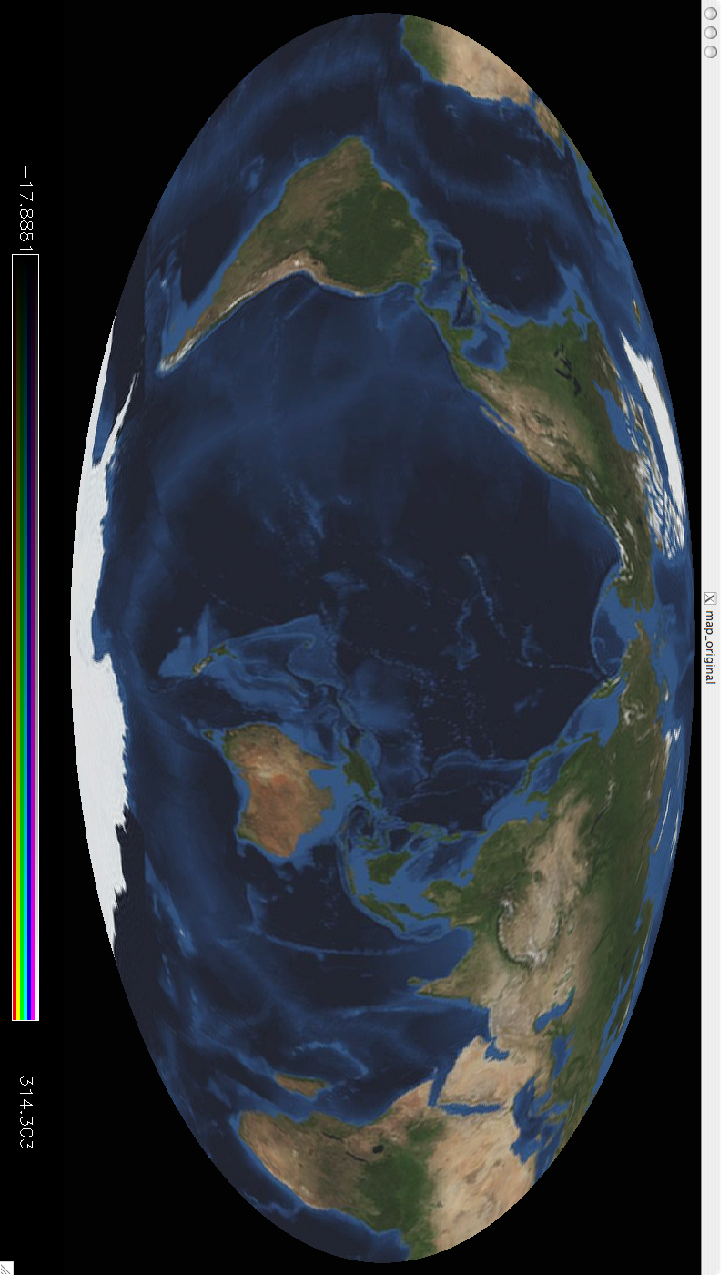
\includegraphics[angle=90,width=8cm]{earth_ori.pdf}
}}
\centerline{
\hbox{
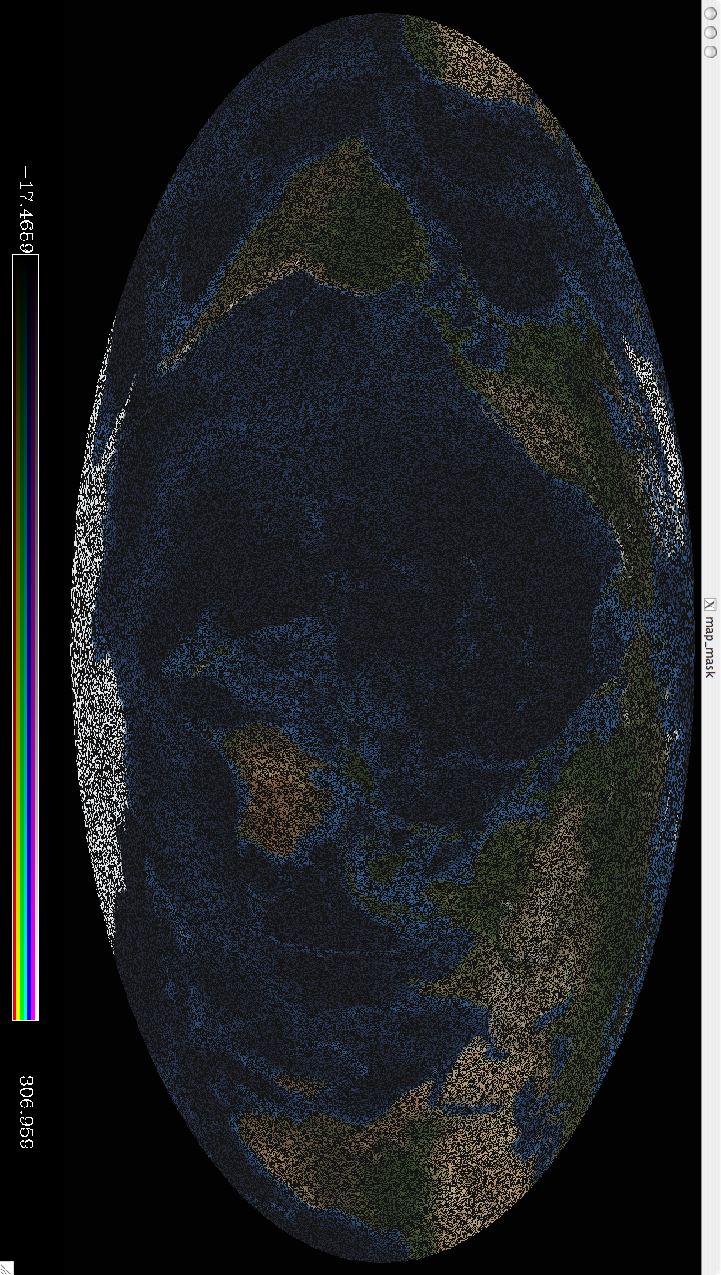
\includegraphics[angle=90,width=8cm]{earth_mask.pdf}
}}
\centerline{
\hbox{
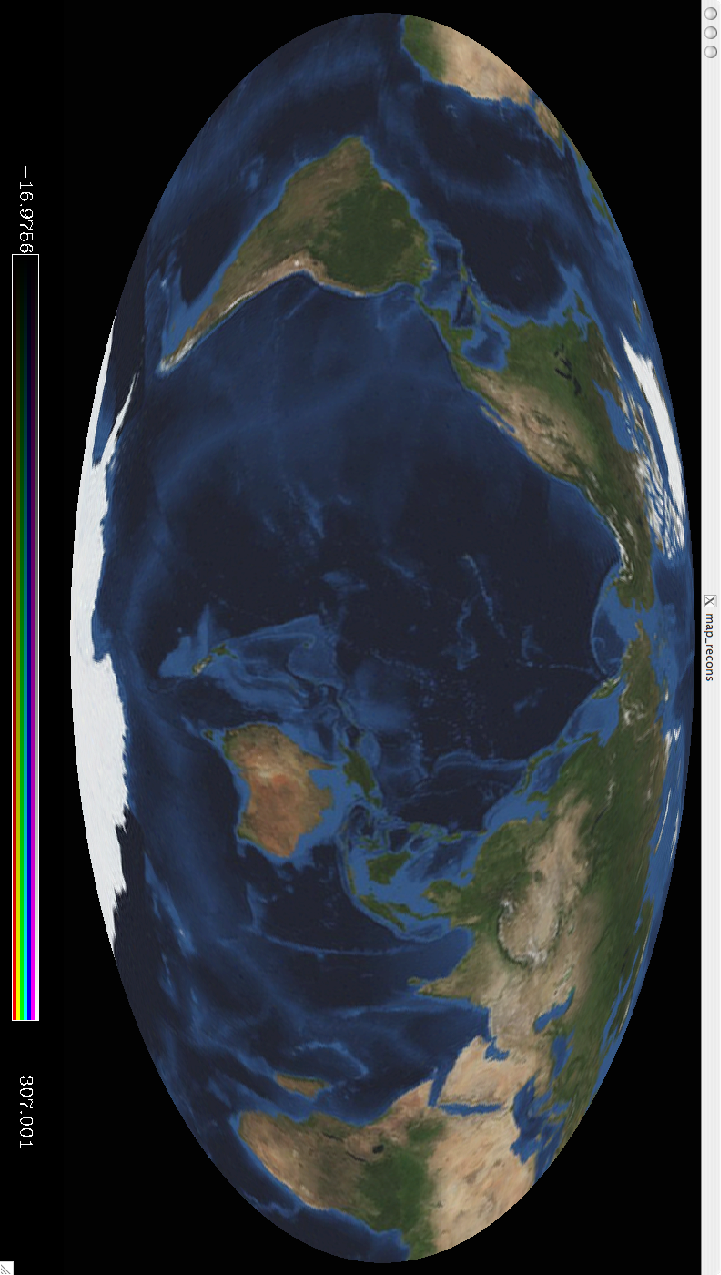
\includegraphics[angle=90,width=8cm]{earth_recons.pdf}
}}
}
 \caption{ Application of the proposed MCA-inpainting algorithm on the sphere. Top: original satellite view of the Earth.  
Middle: incomplete map retaining 40 percent of the original pixels. 
Bottom: inpainted map.}
\label{Figure:mcaearth}
\index{data!Earth}
\end{figure}

A simple numerical experiment is shown in Fig.~\ref{Figure:mcaearth}. 
Starting with a full satellite view of the Earth\footnote{Available from: http://www.nasa.gov/vision/earth/features/bmng\_gallery\_4.html}, 
an incomplete spherical map was obtained by randomly masking some of the pixels. In fact, as much as sixty percent of the pixels were masked. Using both the spherical harmonics transform and the curvelet transform on the sphere within the proposed MCA inpainting algorithm, it is possible to fill in the missing pixels in a visually undetectable way. 

%---------------------------------------------------------------------------------------------------------------------------------------
\newpage
\subsection{Application in Cosmology}
\label{section:cmb}

A major issue in modern cosmology is the measurement and the statistical characterization  (spatial power spectrum, Gaussianity)  of the slight fluctuations in the Cosmic Microwave Background radiation field. These are strongly related to  the cosmological scenarios describing the properties and evolution of our Universe. Some 370,000 years after the Big Bang, when the temperature of the Universe was around 3000~K, thermal energy was no longer sufficient to keep electrons and positively charged particles apart so they combined. Photons were then set free in a nearly transparent Universe. Since the Universe further expanded, these photons are now in the microwave range but they should still be distributed according to a black body emission law. Indeed, before recombination, the Universe was a highly homogeneous opaque plasma in near thermal equilibrium in which photons and charged particles were highly interacting.  Hence the slight fluctuations in matter density, from which such large scale structures as galaxies or clusters of galaxies have evolved, are also imprinted on the distribution of photons.\\
\begin{figure}[htb]
\vbox{
\centerline{
\hbox{
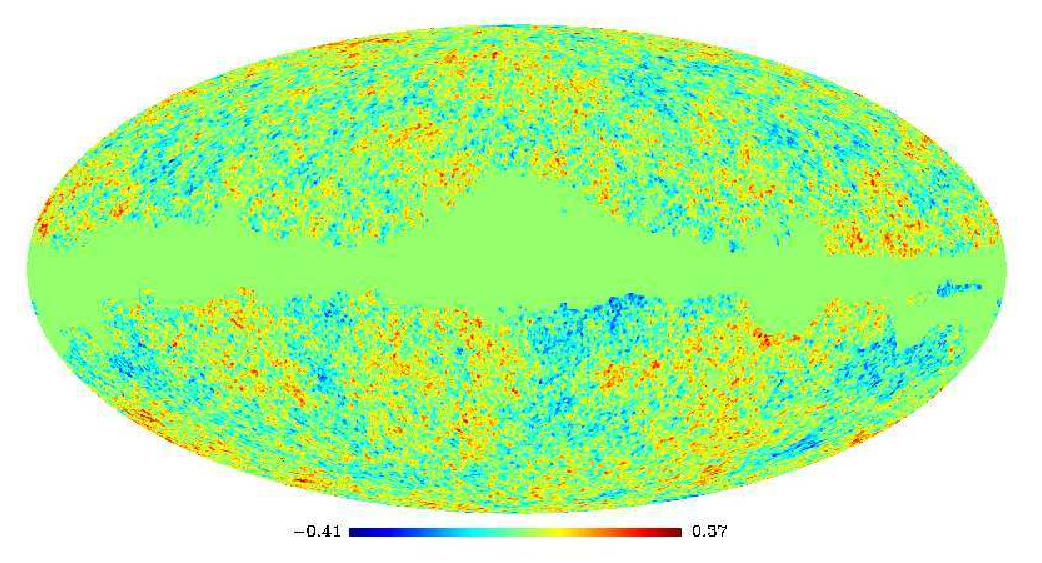
\includegraphics[width = 7.9cm]{ADAIV_poster_abrial_fig1}
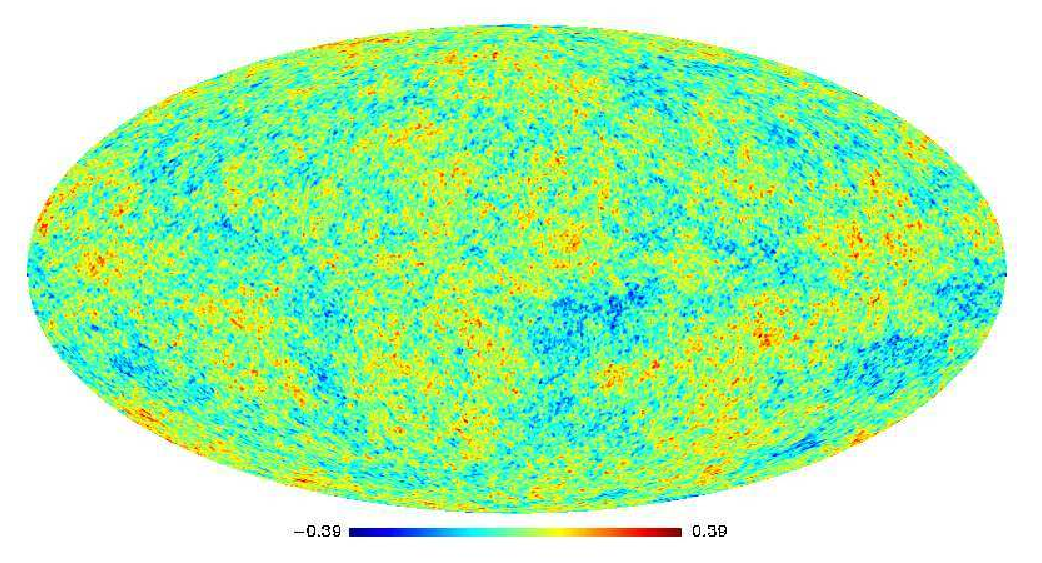
\includegraphics[width = 7.9cm]{ADAIV_poster_abrial_fig2}
}
}
}
\caption{Left: CMB data map provided by the WMAP team. Areas of significant foreground contamination in the galactic region and at the locations of strong radio point sources have been masked out. Right: Map obtained by applying the  MCA-inpainting algorithm on the sphere to the former incomplete WMAP CMB data map.}
\label{cmb_wmap_inpainting}
\index{data!CMB}
\end{figure}

\index{CMB}
\index{Cosmic Microwave Background}
The Cosmic Microwave Background (CMB) was first observed in 1965 by Penzias and Wilson confirming a prediction made by Gamow in the late 1940s. But it was not until the early 1990s that evidence for small fluctuations in the CMB sky could finally be found thanks to the observations made by COBE~\citep{gauss:smoot92}. This was confirmed by several subsequent observations and recently by NASA's Wilkinson Microwave Anisotropie Probe (WMAP) \footnote{The WMAP data and mask we used here are available online at http://map.gsfc.nasa.gov/}. Full-sky multi-spectral observations with unprecedented sensitivity and angular resolution are expected from ESA's Planck\footnote{http://astro.estec.esa.nl/Planck} mission, which was launched in 2009. The statistical analysis of this data set will help set tighter bounds on major cosmological parameters.\\

\begin{figure}[htb]
\vbox{
\centerline{
\hbox{
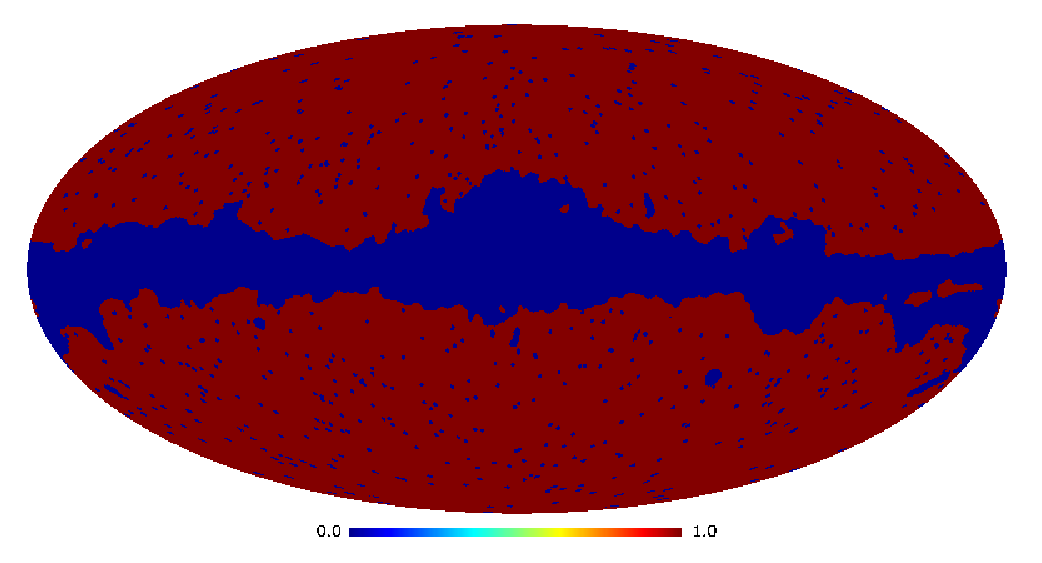
\includegraphics[width=7.9cm]{ADAIV_poster_abrial_fig6}
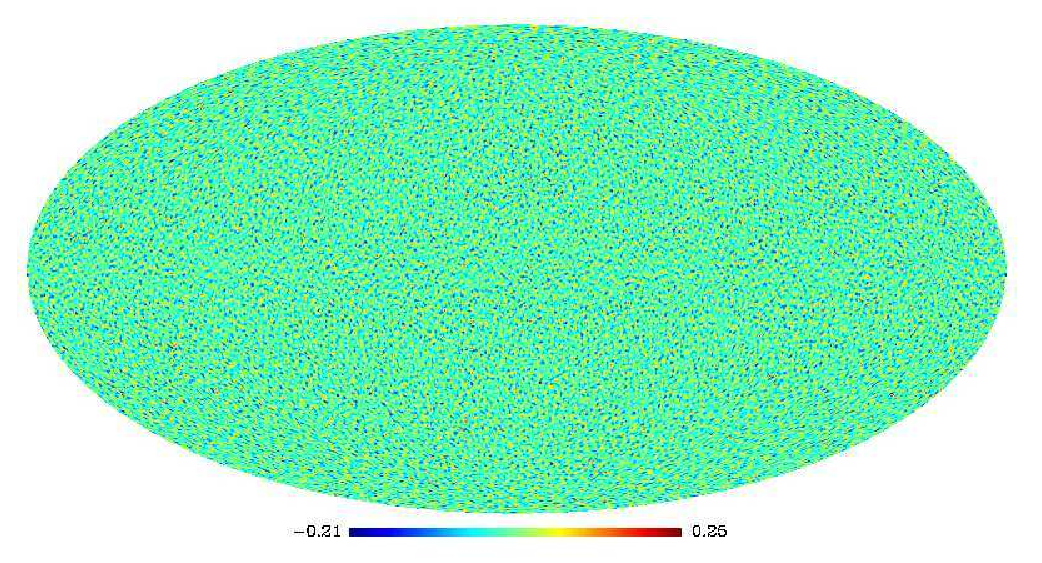
\includegraphics[width=7.9cm]{ADAIV_poster_abrial_fig7}
}
}
\centerline{
\hbox{
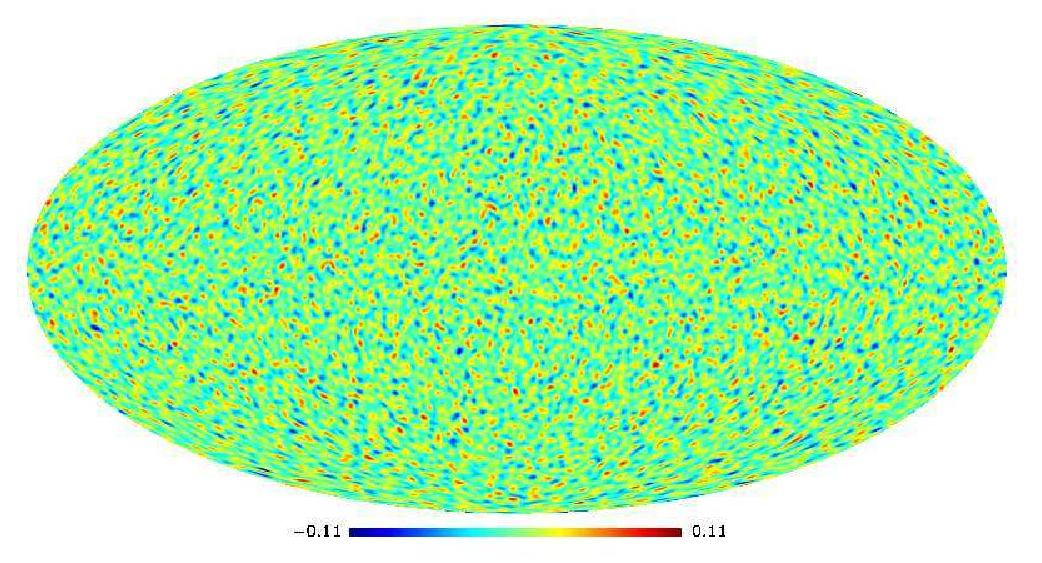
\includegraphics[width=7.9cm]{ADAIV_poster_abrial_fig8}
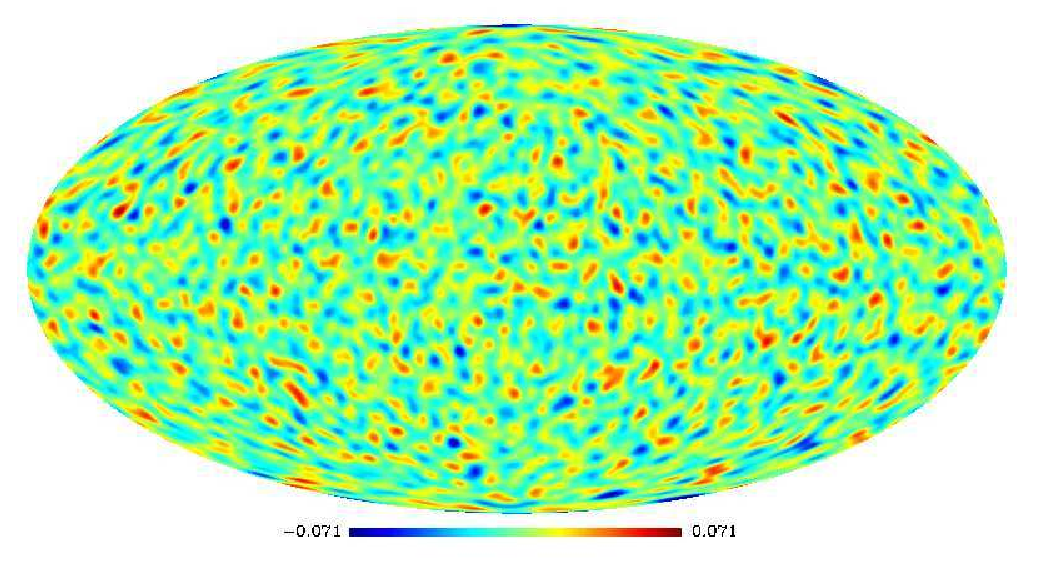
\includegraphics[width=7.9cm]{ADAIV_poster_abrial_fig9}
}
}
\centerline{
\hbox{
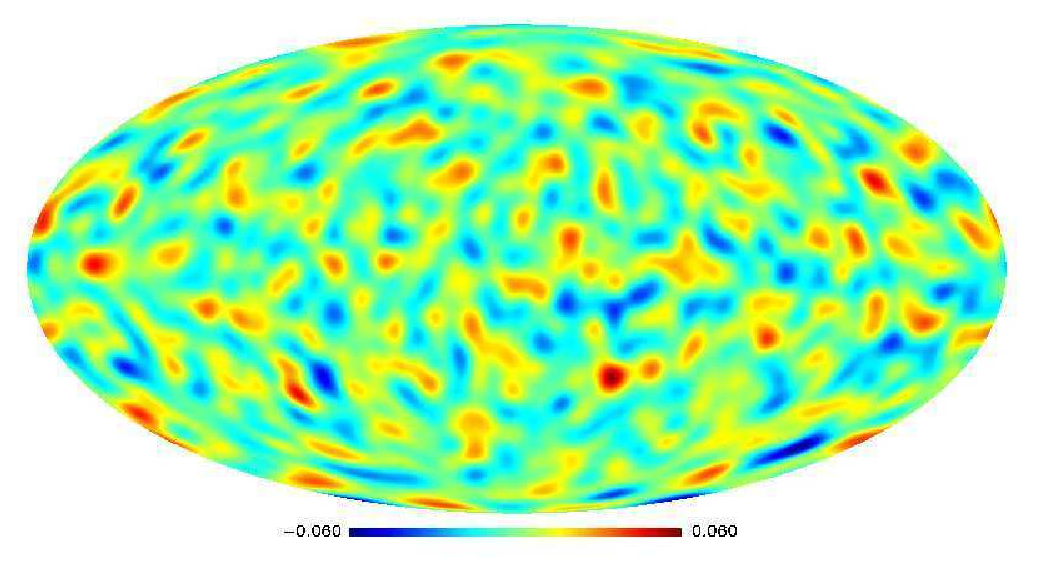
\includegraphics[width=7.9cm]{ADAIV_poster_abrial_fig10}
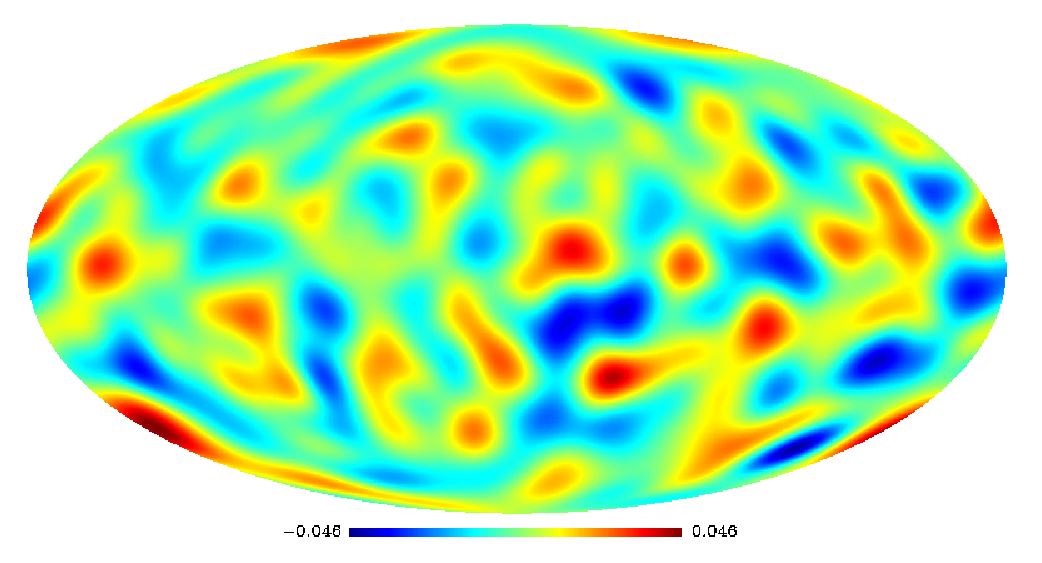
\includegraphics[width=7.9cm]{ADAIV_poster_abrial_fig11}
}
}
\centerline{
\hbox{
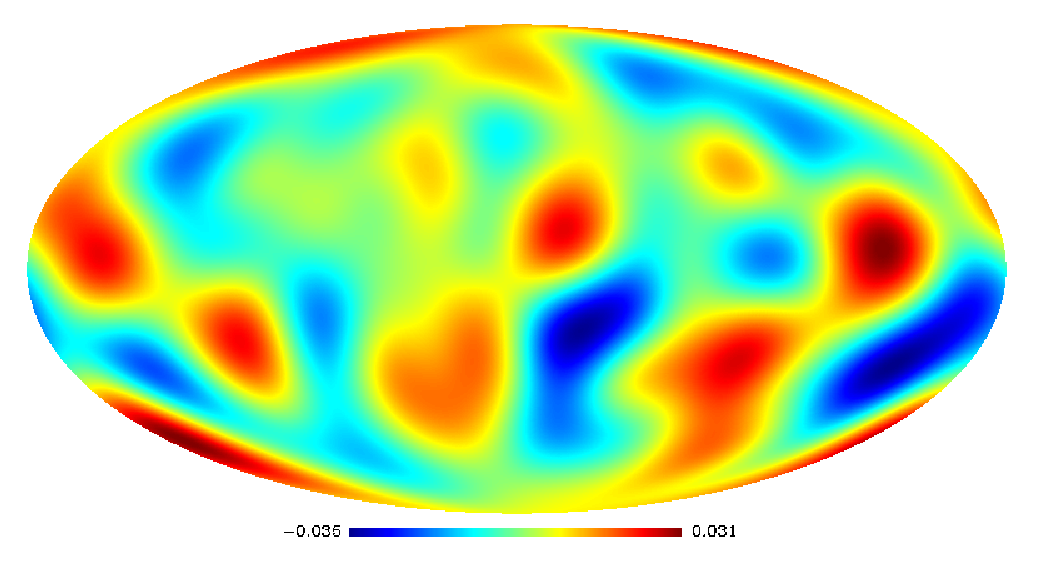
\includegraphics[width=7.9cm]{ADAIV_poster_abrial_fig12}
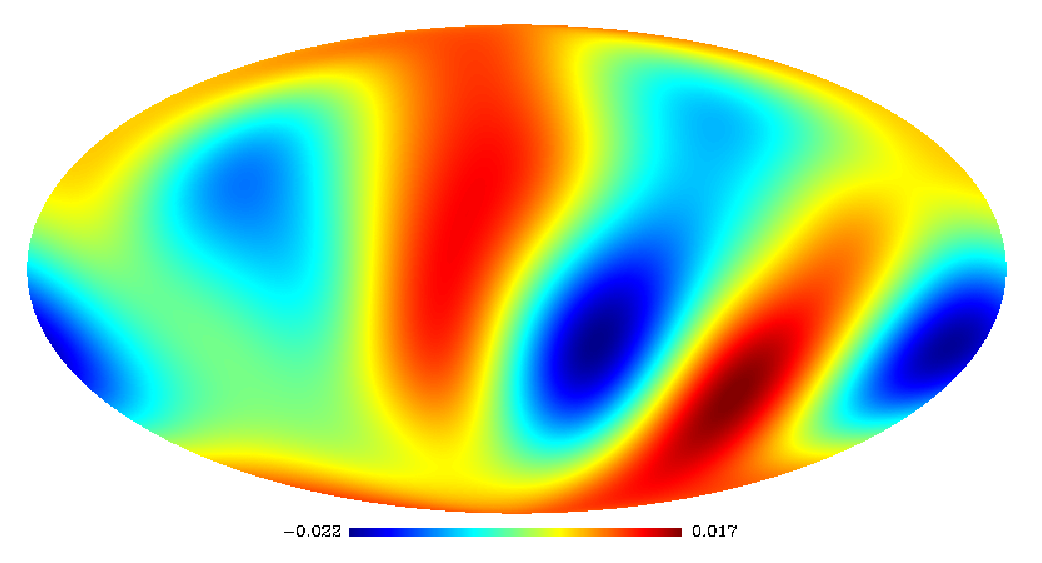
\includegraphics[width=7.9cm]{ADAIV_poster_abrial_fig13}
}
}
}
\caption{Top left: Masked area. From top to bottom and left to right: The seven wavelet scales of the inpainted map. From the visual point  of view, the initially masked area cannot be distinguished any more in the wavelet scales of the inpainted map.}
\label{cmb_scale_wmap_inpainting}
\end{figure}

A simple numerical experiment is shown in Fig.~\ref{cmb_wmap_inpainting}, starting with the full-sky CMB map provided by the WMAP team.
% and available at http://map.gsfc.nasa.gov/. 
This CMB map was partially masked to discard pixels where the level of  contamination by residual foregrounds is expected to be the highest. Applying the described inpainting algorithm, making use of the sparsity of the representation of CMB in the spherical harmonics domain, leads to the map shown on the right of Fig.~\ref{cmb_wmap_inpainting}: the stationarity of the CMB field appears to have been restored and the masked region is completely undetectable to the eye.  Fig.~\ref{cmb_scale_wmap_inpainting} shows the wavelet decomposition of the inpainted map allowing for further visual positive assessment of the quality of the proposed method as again the masked regions are undetectable at all scales. It was shown in \citep{inpainting:abrial06,starck:abrial08} that inpainting the CMB map is an interesting approach for analyzing it, especially for non-Gaussianity studies and power spectrum estimation.


 